\documentclass[a4paper]{article}
\usepackage{geometry}\geometry{a4paper,left=2.5cm,right=2.5cm,top=3cm,bottom=2.5cm}
\usepackage{setspace}\onehalfspacing
\usepackage{fancyhdr}\pagestyle{fancy}\fancyhf{}
\fancyhead[L]{\small A No-Go Theorem for Introspection in Pretrained Generative LLMs}
\fancyhead[R]{\small\thepage}\renewcommand{\headrulewidth}{0.5pt}
\usepackage[colorlinks=true,linkcolor=blue]{hyperref}
\usepackage{amsmath,amssymb,mathtools}
\usepackage{seqsplit}
\allowdisplaybreaks
\sloppy
\emergencystretch=2em
\usepackage{tikz}\usetikzlibrary{calc,shadows,fadings,decorations.pathmorphing,patterns,backgrounds,arrows.meta,positioning}
\usepackage{pgfplots}\pgfplotsset{compat=1.17}
\usepackage{xcolor,titlesec,enumitem}
\definecolor{fo}{RGB}{255,120,20}\definecolor{fy}{RGB}{255,200,50}
\definecolor{fr}{RGB}{220,40,20}\definecolor{db}{RGB}{10,10,20}
\definecolor{sb}{RGB}{40,80,140}\definecolor{gd}{RGB}{200,160,40}
\definecolor{redColor}{RGB}{227,0,26}
\definecolor{greenColor}{RGB}{0,120,31}
\definecolor{grayColor}{RGB}{32,32,32}
\definecolor{TitleGreen}{RGB}{0,120,55}
\usepackage{graphicx}
\usepackage{array}
\usepackage{listings}
\usepackage{booktabs}
\usepackage{multirow}

% ---- listings configuration ----
\definecolor{codebg}{RGB}{248,248,252}
\definecolor{codeframe}{RGB}{200,200,220}
\lstset{
  basicstyle=\footnotesize\ttfamily,
  backgroundcolor=\color{codebg},
  frame=single,
  rulecolor=\color{codeframe},
  framerule=0.5pt,
  breaklines=true,
  numbers=left,
  numberstyle=\tiny\color{gray},
  numbersep=5pt,
  tabsize=2,
  showstringspaces=false,
  keywordstyle=\color{sb}\bfseries,
  commentstyle=\color{grayColor}\itshape,
  stringstyle=\color{redColor},
  captionpos=b,
  aboveskip=8pt,
  belowskip=8pt,
}
\titleformat{\section}{\normalfont\Large\bfseries\sffamily\color{sb}}{\thesection}{1em}{}
\titleformat{\subsection}{\normalfont\large\bfseries\sffamily\color{sb!80}}{\thesubsection}{1em}{}
\titleformat{\subsubsection}{\normalfont\normalsize\bfseries\sffamily\color{sb!60}}{\thesubsubsection}{1em}{}

% Frequently used mathematical notation
\newcommand{\R}{\mathbb{R}}
\newcommand{\N}{\mathbb{N}}
\newcommand{\E}{\mathbb{E}}
\newcommand{\norm}[1]{\left\lVert #1 \right\rVert}
\newcommand{\abs}[1]{\left\lvert #1 \right\rvert}
\newcommand{\sgn}{\operatorname{sgn}}
\newcommand{\KL}[2]{D_{\mathrm{KL}}\!\left(#1\,\|\,#2\right)}
\newcommand{\TV}[2]{d_{\mathrm{TV}}\!\left(#1,#2\right)}
\newcommand{\supp}{\operatorname{supp}}
\newcommand{\doop}{\operatorname{do}}
\newcommand{\indep}{\perp\!\!\!\perp}

% ---- Theorem environments (numbered in the style ``X.Y.Z'') ----
\usepackage{amsthm}
\newtheoremstyle{cnplain}{10pt}{10pt}{\normalfont}{0pt}{\bfseries\color{sb}}{.}{.5em}{}
\newtheoremstyle{cndef}{10pt}{10pt}{\normalfont}{0pt}{\bfseries\color{sb!80}}{.}{.5em}{}
\theoremstyle{cnplain}
\newtheorem{theorem}{Theorem}
\newtheorem{corollary}{Corollary}
\newtheorem{lemma}{Lemma}
\theoremstyle{cndef}
\newtheorem{definition}{Definition}
\newtheorem{assumption}{Assumption}
\newtheorem{remark}{Remark}
\newtheorem{example}{Example}
\newtheorem*{proposition}{Proposition}
\newtheorem*{restate}{Theorem}
\newtheorem*{restatecor}{Corollary}
\renewcommand{\proofname}{Proof}

\title{\bfseries\Large Introspective Capacity of Pretrained Generative Language Models:\\[2pt]
A No-Go Theorem under Static Pretraining and Autoregressive Generation}
\author{Sheng Cheng\textsuperscript{a,*}\\
\normalsize\textsuperscript{a} Hefei Jiuzhai Big Data Technology Co., Ltd., Hefei, China\\
\normalsize\textsuperscript{*} Corresponding author. E-mail: c.sheng@cumt.edu.cn}
\date{\today}

\begin{document}
\maketitle

\begin{abstract}
\noindent This paper provides a mathematical proof of the following proposition $P$:
within the technical paradigm $\Pi$, namely Transformer architecture + static pretraining +
autoregressive generation, no pretrained generative large language model possesses
\textbf{introspective capacity in the human sense}.

\medskip
\noindent ``Introspection in the human sense'' is operationalized as five necessary criteria
($\mathrm{A}_1$--$\mathrm{A}_5$): accuracy (the self-report agrees with the system's true
internal state), grounding (the self-report depends causally on the state it reports),
internality (that causal dependence does not pass through the system's own sampled outputs),
metacognitive representation (the system registers, before reporting, the second-order fact
``I am in state $s$''), and closed-loop plasticity (an introspective event can change the
system's future internal state through a \textbf{private} channel, not merely through public
text).

\medskip
\noindent Under explicit assumptions ($\Pi_1$--$\Pi_5$) this paper proves six theorems.
\textbf{Theorem 1} (absence of an introspective information channel): under the paradigm's
sampling model, the report $R$ and the hidden state $H$ are conditionally independent given
the public pair $(\theta,c)$, i.e., $I(R;H\mid\theta,c)=0$; the training objective provides
no supervision for the ``ground-truth introspection mapping'', so introspective accuracy admits
\textbf{no nontrivial PAC-style guarantee} (otherwise contradicting the No-Free-Lunch
theorem). \textbf{Theorem 2} (proxy-objective mismatch): the text-likelihood objective is
statistically orthogonal to the introspective target ($O^{*} \indep D \mid \theta$); under
the absence of state labels ($\Pi_5$), maximizing text likelihood does \textbf{not
constrain}, and can strictly harm, introspective accuracy (a strict instantiation of Goodhart
regression). \textbf{Theorem 3} (closed-loop failure): frozen weights at inference ($\Pi_2$)
imply that the system possesses no private self-update channel independent of the public text
channel; all ``self-influence'' must pass through the context channel, whose information content
is bounded above by $C\log\abs{\Sigma}$ bits. \textbf{Theorem 4} (generation is not
verification): paradigm $\Pi$ implements only the sampling kernel $p_\theta$, not a grounding
verifier; a model's judgment of whether its own statement is ``grounded'' is itself a sample of
corpus statistics, not an evaluation of truth. \textbf{Theorem 5} (no privileged channel):
every report can be reproduced by any third party holding $(\theta,c)$ at equal computational
cost, so the ``privileged self-access'' criterion fails; moreover, there exist hidden-state
description functions that an external probe reads exactly yet the model cannot reliably
report through its text channel. \textbf{Theorem 6} (no self-model evolution): the self-model
$g_\theta$ is a constant function throughout inference; the growth of runtime
``self-knowledge'' is doubly capped by the context window $C$ and the frozen kernel $p_\theta$.

\medskip
\noindent It follows that, within paradigm $\Pi$, any system can achieve at most \textbf{weak
functional self-report}: accuracy unguaranteed, ungrounded in the native generative regime,
no private closed loop, no privileged channel, and unable to drive self-model evolution. The
empirical findings of the Anthropic concept-injection paper (arXiv:2601.01828), with a
success rate of about 20\%, strong context dependence, zero net benefit for base models, an
unverifiable metacognitive-representation criterion, and an explicit denial of human-like
self-awareness, agree completely with the theorems above and are, to a large extent, their
necessary corollaries.

\medskip
\noindent The paper also draws its boundaries precisely: every impossibility theorem
presupposes paradigm $\Pi$; once any pillar is relaxed (online plasticity, a non-static
corpus, a non-textual interface, an explicit verifier), the corresponding theorems cease to
hold. Accordingly, this paper does \textbf{not} support the absolutist claim ``never'', but
only ``impossible within the current paradigm'', which is exactly the precise content of
proposition $P$.

\medskip
\noindent\textbf{Keywords}: introspection; autoregressive large language models; static
pretraining; information theory; computational learning theory; No-Free-Lunch theorem;
Goodhart's law; causal inference; metacognition
\end{abstract}

\clearpage

% ══════════════════════════════════════════════════════════════════
\section{Introduction}

\subsection{Background and Significance}

In January 2026, the Anthropic research team published the paper
\emph{Emergent Introspective Awareness in Large Language Models}
(arXiv:2601.01828)\cite{lindsey-2026-introspection}, which systematically examines large
language models' (LLMs) ability to self-report their own internal states through
\textbf{concept injection}. The core experimental paradigm is as follows: an activation
vector encoding a specific concept is injected into the model's residual stream, and the model
is then asked whether it ``noticed'' the injected ``thought''. The authors report several striking
qualitative results: Claude Opus 4.1, for example, can sometimes ``notice'' an injected concept
before producing any output, can distinguish ``thoughts'' from textual input, and, in the
prefill-detection experiment, judges whether a given output was ``intentional'' on the basis of
prior activations. At the same time, the authors impose a series of important caveats: the
success rate is only about 20\%, failure is the norm, the mechanism may be shallow and narrow,
the experimental setup is unnatural, and they \textbf{explicitly disclaim} that the models
possess human-like self-awareness or subjective experience\cite{lindsey-2026-introspection}.

This paper and the discussion it generated have, for the first time, placed the question
``can large language models introspect?'', a question long confined to the philosophical and
phenomenological level, on an intervenable and reproducible causal experimental platform.
Yet however compelling they may be qualitatively, empirical findings cannot directly answer
a more fundamental mathematical question:

\begin{quote}
\itshape
Within the paradigm $\Pi$ adopted by nearly all current frontier models, namely
\textbf{Transformer architecture + static pretraining + autoregressive generation}, can a
pretrained generative model possess human-significance introspective capacity \textbf{in
principle}?
\end{quote}

``In principle'' means: independent of the contingent implementation details of any particular
model (a specific layer, a specific injection strength, a specific prompt), we ask whether the
paradigm $\Pi$ itself imposes structural constraints. If there exist insurmountable
mathematical obstacles at the paradigm level, then any experimental ``success case'' can only be
a by-product of inductive bias rather than a structural capacity. Conversely, if no obstacle
exists at the paradigm level, then the experimentally observed low success rate is merely an
engineering-scale issue.

The contribution of this report is \textbf{to formalize the term ``introspection'' with
rigorous mathematical tools (information theory, computational learning theory, algorithmic
information theory, causal inference), and to prove that paradigm $\Pi$ fails structurally on
five necessary criteria for human-significance introspection}. The proof serves two purposes:
it gives proposition $P$ (see Section 1.5) a deductive basis, and it marks out precise
boundary conditions for architectures that might in the future transcend the paradigm
(online learning, embodied interaction, explicit verifiers, and so on).

\subsection{Related Work}

\subsubsection{The Definitional Debate over Introspection}

The definition of ``introspection'' is itself contested. Kammerer and Frankish
define introspection as ``the process by which a cognitive system represents its own current
mental states, with this information being usable for online behavioral control''
\cite{kammerer-frankish-2023}; Long applies this functional definition to large language
models\cite{long-2023-introspection}; Comsa and Shanahan emphasize causality: ``an LLM
self-report is introspective if and only if it accurately describes an internal state of the
LLM through a causal process that links the internal state and the self-report''
\cite{comsa-shanahan-2025}; Song et al.\ criticize the above definitions for failing to
highlight \textbf{privileged self-access}, proposing instead that introspection is ``any process
which yields information about internal states of the AI through a process that is more
reliable than any process with equal or lower computational cost available to a third party
without special knowledge of the situation'' (paraphrased)\cite{song-privileged-2025}.

Lindsey, in arXiv:2601.01828, adopts four operational criteria\cite{lindsey-2026-introspection}:
(1) \textbf{Accuracy}: the self-report must be accurate; (2) \textbf{Grounding}: the
self-report must causally depend on the state it describes; (3) \textbf{Internality}: that
causal dependence must not pass through the model's already-sampled outputs;
(4) \textbf{Metacognitive representation}: the self-report must arise from an internal
second-order representation of the state itself, rather than a direct translation of the
state. The authors concede that criterion (4) cannot be directly verified in their
experiments.

\subsubsection{Concept Injection and Causal Experiments}

Concept injection (activation steering) originates from Representation
Engineering\cite{zou-2023-repeng} and Activation Addition\cite{turner-2023-actadd}. The SelfIE
work of Chen et al.\cite{chen-2024-selfie} and the Patchscopes work of Ghandeharioun et
al.\cite{ghandeharioun-2024-patchscopes} ``transplant'' activations produced under one prompt
into a blank position of another prompt, letting the model ``say'' what the activation means.
The work of Ji-An et al.\ shows that models can, guided by in-context examples, report and
regulate the projection of their activations along specified probe directions
\cite{ji-an-2025-metacog}. On top of these techniques, Lindsey's work introduces
\textbf{interventional causal adjudication}: by altering the internal state and observing
whether the self-report changes accordingly, one adjudicates grounding. This brings
Rubin/do-calculus-style causal thinking\cite{pearl-2009} into introspection experiments
in a systematic way.

\subsubsection{Self-Modeling and Meta-Knowledge}

A separate line of research, distinct from ``introspecting one's own activations'',
examines models' prediction of \textbf{their own behavior}. The situational awareness dataset (SAD) of
Laine et al.\ shows that some models can predict their own outputs reasonably
well\cite{laine-2024-sad}; Binder et al.\ find that fine-tuned models predict their own
behavior better than others' behavior\cite{binder-2024-looking-inward}; Kadavath et al.\ show
that, with appropriate prompting, models' answer probabilities are well calibrated with
correctness\cite{kadavath-2022-know}; Cheng et al.\ train assistants, using model-specific
datasets, to refuse questions they cannot answer correctly\cite{cheng-2024-know-gaps}; Ferrando
et al.\ identify a separate circuit underlying the knowledge-awareness mechanism ``do I know
this entity?''\cite{ferrando-2024-know-entity} (Lindsey et al.'s biological analysis likewise
observes the independence of this mechanism\cite{lindsey-2025-biology}); Betley et al.\ show
that models can describe behavioral propensities acquired through fine-tuning
\cite{betley-2025-propensities}; Plunkett et al.\ further show that models can quantitatively
report the internal weights that drive their decisions\cite{plunkett-2025-self-interp}; Wang et
al.\ reproduce propensity introspection with steering vectors\cite{wang-2025-out-of-context};
Davidson et al., using a different set of prompts, find no evidence of consistent
self-recognition\cite{davidson-2024-selfrecog}. Song et al.\ question several of the above
conclusions, arguing that many ``self-prediction'' effects can be attributed to similarity
between models rather than privileged access\cite{song-2025-introspect-language}.

\subsubsection{Nascent Mathematicization}

Work that casts LLM limitations as theorems has only just begun. Kalai and Vempala prove that
\textbf{calibrated language models must hallucinate}: if a language model's conditional
probabilities are calibrated (the model's reported confidence equals its actual correctness),
then, whenever unavoidable ignorance points exist, it must give wrong answers on some open
queries; it is one of the few rigorous results that explains, at the level of the objective
function, the tension between ``generative distribution'' and ``truth''
\cite{kalai-vempala-2023-calib}; Kalai et al.\ provide further theoretical analysis of the
mechanisms behind hallucination\cite{kalai-2025-hallucinate}. Skalse et al.\ systematically
characterize the mathematical structure of ``reward hacking / proxy-objective mismatch''
\cite{skalse-2022-reward-hacking}, and Manheim and Garrabrant formalize a taxonomy of
Goodhart's-law variants\cite{manheim-garrabrant-2018-goodhart}. These tools provide the
mathematical language used here. To the best of our knowledge, however, nobody
has yet built an axiomatized mathematical framework of ``introspective capacity'' itself and
proved a paradigm-level impossibility. This is the gap the present report fills.

\subsection{Limitations of Existing Work}

The literature above has three limitations:

\begin{enumerate}
\item \textbf{Lack of paradigm-level formalization.} Existing discussion (including
arXiv:2601.01828 itself) is bounded by ``what experiments can observe''; it does not answer
``what the paradigm $\Pi$ structurally permits''. The experimentally observed 20\% success rate
can be explained by arbitrarily many mechanisms (the paper's own authors list several
``simplest mechanism'' conjectures\cite{lindsey-2026-introspection}), but no theorem states
\textbf{why} the success rate could not be pushed near 100\% by some clever training recipe,
or, conversely, \textbf{why} certain introspective criteria cannot possibly be satisfied within
the paradigm.
\item \textbf{Lack of logical relations among criteria.} The paper's four criteria are given
in parallel, without arguing for their necessity, sufficiency, or their coupling to the
paradigm structure. For example, ``internality'' and ``privileged access'' (emphasized by Song et
al.\cite{song-privileged-2025}) both derive from the same mathematical fact, namely that the report is a
public function of $(\theta,c)$, yet existing literature does not unify them.
\item \textbf{Failure to distinguish ``statistical correlation'' from ``structural guarantee''.}
The causal association ``internal representation $\to$ self-report'' established by concept
injection experiments is established under \textbf{external intervention}. Whether any
information channel exists between report and state in the \textbf{native generative regime}
of paradigm $\Pi$ (no intervention) is a question that has never been rigorously examined.
Theorem 1 below will prove: in the native regime the information content of that
channel is zero ($I(R;H\mid\theta,c)=0$).
\end{enumerate}

\subsection{Research Content and Contributions}

The research content of this report is to formalize ``introspection in the human sense'' as
five necessary criteria ($\mathrm{A}_1$--$\mathrm{A}_5$), to formalize the paradigm $\Pi$ as
five structural postulates ($\Pi_1$--$\Pi_5$), to prove six impossibility theorems, to test
them against the empirical findings of arXiv:2601.01828, and finally to delimit the scope of
the theorems.

The contributions are summarized as follows:

\begin{itemize}
\item \textbf{Axiomatization}: the first five-criterion formalization of ``introspection''
(merging the paper's four criteria with Kammerer--Frankish online control, Song's privileged
access, and closed-loop plasticity); every criterion is a testable mathematical condition.
\item \textbf{Paradigm characterization}: distilling ``Transformer + static pretraining +
autoregressive generation'' into five postulates, so that ``paradigm-level impossibility''
becomes a provable proposition rather than an intuitive judgment.
\item \textbf{Six theorems}: the information-gap theorem, the proxy-objective-mismatch theorem,
the closed-loop-failure theorem, the generation--verification separation theorem, the
no-privileged-channel theorem, and the no-self-model-evolution theorem. Theorems 1, 2, 3, 5
are rigorous proofs (grade A); Theorems 4 and 6 are structural assertions with heuristic
arguments (grades A/B); complete proofs of all theorems are given in Appendix A.
\item \textbf{Boundary analysis}: a precise correspondence table of ``which theorem fails when a
given postulate is relaxed'', strictly confining the ``impossibility'' claim to paradigm $\Pi$ and
avoiding absolutism.
\end{itemize}

\subsection{Statement of the Proposition and Proof Strategy}

\subsubsection{Precise Statement of the Proposition}

\begin{proposition}[Master Proposition $P$ (the proposition proved below)]
Within the paradigm $\Pi$ (Assumption \ref{asm:paradigm}), there exists no system obtained by
static pretraining plus autoregressive generation that satisfies the five necessary criteria
$\mathrm{A}_1$--$\mathrm{A}_5$ of human-significance introspection (Definition
\ref{def:criterion}).
\end{proposition}

Note the two qualifiers of proposition $P$: (i) \textbf{``within the paradigm $\Pi$''},
which excludes all out-of-paradigm implementations such as online learning, non-textual
interfaces, and explicit verifiers; (ii) \textbf{``in the human sense''}, meaning that the criteria
$\mathrm{A}_1$--$\mathrm{A}_5$ are operationalized necessary conditions that span
consciousness theories (Section 5.2 will argue their necessity), but no commitment is made
here to any phenomenological (qualia) conclusion.

\subsubsection{Overview of the Proof Strategy}

The proof proceeds in four steps.

\begin{enumerate}
\item \textbf{Formalization (Chapter 2)}: give the paradigm postulates $\Pi_1$--$\Pi_5$, the
system state model, and the mathematical definitions of the five introspective criteria
$\mathrm{A}_1$--$\mathrm{A}_5$.
\item \textbf{Theorems (Chapter 3)}: prove the six theorems one by one. The conclusion of each
theorem maps to the failure of at least one criterion (see Table \ref{tab:thm-criteria}).
\item \textbf{Empirical testing (Chapter 4)}: test the theorems' predictions against the
quantitative results of arXiv:2601.01828, showing that the ``weak functional self-report''
observed by the paper is a necessary corollary of the theorems.
\item \textbf{Boundaries (Chapter 5)}: argue that proposition $P$ does not invert:
out-of-paradigm architectures are not constrained by the theorems, and the absolutist claim
``never'' does not hold.
\end{enumerate}

\begin{table}[htbp]
\centering
\caption{Correspondence between the six theorems and the five criteria (overview)
\label{tab:thm-criteria}}
\begin{tabular}{p{2.0cm}p{5.4cm}p{5.4cm}p{1.4cm}}
\toprule
Theorem & Content & Criterion failed & Grade \\
\midrule
Theorem 1 & Absence of an introspective information channel & $\mathrm{A}_1$ (no accuracy guarantee) & A \\
Theorem 2 & Proxy-objective mismatch & $\mathrm{A}_1$ (objective unrelated) & A \\
Theorem 3 & Closed-loop failure & $\mathrm{A}_5$ (no private closed loop) & A \\
Theorem 4 & Generation $\neq$ verification & $\mathrm{A}_4$ (metarepresentation unguaranteed) & A/B \\
Theorem 5 & No privileged channel & $\mathrm{A}_3$ (internality/privileged access fails) & A \\
Theorem 6 & No self-model evolution & $\mathrm{A}_5$ (no self-correction) & A/B \\
\bottomrule
\end{tabular}
\end{table}

\subsubsection{Grading Statement}

Following the principle of academic honesty, all assertions in this report are graded.
\textbf{Grade A} marks theorems strictly provable under the explicit postulates; \textbf{Grade B}
marks structural assertions with heuristic arguments (their mathematical core is grade A, but
their interpretation for real systems relies on additional assumptions); \textbf{Grade C} marks
architectural judgments; \textbf{Grade D} marks philosophical assumptions (e.g., ``the five
criteria are necessary conditions for human introspection''). The complete grading table is in
Section 6.3, and complete proofs are in Appendix A.

\section{Formal Framework}

This chapter establishes all mathematical objects needed for the subsequent proofs. We
define, in order: the paradigm postulates, the system state model, the formalization of the
introspective criteria, and the measurement tools.

\subsection{Axiomatization of the Paradigm \texorpdfstring{$\Pi$}{Pi}}

\begin{assumption}[Paradigm postulates $\Pi_1$--$\Pi_5$]\label{asm:paradigm}
Let $\Sigma$ be a finite vocabulary (token vocabulary) and $\Sigma^{*}$ the set of finite
strings. \textbf{Paradigm $\Pi$} is characterized by the following five postulates. A
\textbf{paradigm instance} is a quintuple $\mathcal{I}=(\Sigma, D, A, p, C)$ satisfying all
postulates:

\begin{enumerate}[align=left, labelwidth=!, labelsep=0.8em, leftmargin=!, itemindent=0pt]
\item[($\Pi_1$)\textbf{Static pretraining}] The training corpus $D \subseteq \Sigma^{*}$ is
fixed before training begins and does not change during training or inference. The parameters
$\theta = A(D) \in \Theta \subseteq \R^{P}$ are determined once and for all by a training
algorithm $A$ (e.g., stochastic gradient descent on the next-token log-likelihood). The input
to $A$ is only $D$; it contains no runtime state.
\item[($\Pi_2$)\textbf{Frozen at inference}] The parameters are constant during inference:
$\theta(t) = \theta(0)$ for all times $t$. The system has no runtime update mechanism for
$\theta$ (no online learning, no plasticity, no weight evolution).
\item[($\Pi_3$)\textbf{Autoregressive decoding}] The system's outputs are sampled
autoregressively from the conditional probability kernel
$p_\theta: \Sigma^{*} \times \Sigma^{*} \to [0,1]$:
\begin{equation}
p_\theta(y_{1:T} \mid c) = \prod_{t=1}^{T} p_\theta\!\left(y_t \mid c, y_{1:t-1}\right),
\label{eq:autoregressive}
\end{equation}
where $c$ is the context. The context evolves by the \textbf{concatenation law}:
$c_{t+1} = c_t \| y_t$, and at any time $\abs{c_t} \le C$ ($C$ being the context window
length).
\item[($\Pi_4$)\textbf{No explicit verifier}] The inference computation graph implements only
the sampling kernel $p_\theta$. No additional component $V$ exists for adjudicating the truth
of the model's own statements about its internal state.
\item[($\Pi_5$)\textbf{Absence of state labels}] The training corpus $D$ contains no pair of
the form $(c,\, \mathrm{desc}(\Phi_\theta(c)))$, where $\Phi_\theta(c)$ is the activation
state of the model on context $c$ \textbf{after training}, and $\mathrm{desc}$ is an arbitrary
state-description encoding. In other words, the training signal is orthogonal to the target
``reports about this model's own states''.
\end{enumerate}
\end{assumption}

\begin{remark}[Status and verifiability of the postulates]
$\Pi_1$--$\Pi_4$ are factual descriptions of the engineering practice of current mainstream
pretrained models (GPT, Claude, Gemini; the Transformer architecture is described in
\cite{vaswani-2017-attention}, autoregressive pretraining in \cite{brown-2020-gpt3}, and
scaling laws in \cite{kaplan-2020-scaling, hoffmann-2022-chinchilla}); $\Pi_5$ is a logical
consequence of $\Pi_1$: the activation state of the trained model did not exist at training
time and hence cannot appear in a static corpus (the intermediate activations observed during
training do not belong to $D$, and they pertain to the then-current parameters $\theta_t$
rather than to the final $\theta$). $\Pi_5$ may also be regarded as an independent postulate,
so that the relaxation scenario ``state labels are added to the corpus'' can be studied
separately (Section 5.1).
\end{remark}

\subsection{The Underlying Mathematical Structure of the Paradigm}

The postulates of Section 2.1 are abstractions. This section examines the concrete
mathematical structure that the three pillars (the Transformer architecture, static
pretraining, and autoregressive generation) impose on any system within the paradigm, and
states the structural facts on which the impossibility theorems of Chapter 3 rest. None of
the facts below is a new assumption; each is a consequence of the postulates together with
the standard mathematical description of the architecture.

\subsubsection{The Transformer as a static function class}

A Transformer of $L$ layers computes on a shared \textbf{residual stream} of dimension
$d$: each layer adds attention and MLP contributions to the stream,
\begin{equation}
x_{l+1} \;=\; x_l \;+\; \sum_{h=1}^{H} \mathrm{Att}_h(x_l) \;+\; \mathrm{MLP}_l(x_l),
\qquad l = 0, \dots, L-1 ,
\label{eq:residual}
\end{equation}
where each attention head performs a data-dependent kernel average
\begin{equation}
\mathrm{Att}_h(x)_i \;=\; \sum_{j} \alpha_{ij}^{h}\, W_V^{h} x_j,
\qquad \alpha_{ij}^{h} = \frac{\exp\!\left( \langle W_Q^{h} x_i,\, W_K^{h} x_j \rangle / \sqrt{d_h} \right)}
{\sum_{j'} \exp\!\left( \langle W_Q^{h} x_i,\, W_K^{h} x_{j'} \rangle / \sqrt{d_h} \right)},
\label{eq:attention}
\end{equation}
i.e., a softmax-normalized (hence convex) combination of value vectors, with the weights
$\alpha^{h}$ depending on the query-key similarity (a learned kernel smoother over the
context)\cite{elhage-2021-circuits, vaswani-2017-attention}. The hidden state of Definition
\ref{def:forward} is the residual vector at a designated layer: $H_c = x_{l^{*}}(\theta, c)$.

Three structural facts follow directly.

\textbf{(S1) $\Phi_\theta$ is a fixed Lipschitz map.} Every sub-operation of the network is
Lipschitz-continuous with a constant controlled by the weight norms: softmax attention is a
convex combination (nonexpansive), layer normalization normalizes, and the MLP and position
embeddings have bounded weights. Consequently the composition $\Phi_\theta$ is Lipschitz
with a constant $L(\theta)$ bounded by a product of layer constants, and by $\Pi_2$ it is
a \textbf{fixed} function after training. The hidden state $H_c = \Phi_\theta(c)$ is a
deterministic point in $\R^{d}$; there is no stochastic state, no state transition beyond
the concatenation law, and no dependence of $H$ on anything other than $(\theta, c)$.

\textbf{(S2) The residual stream is the only internal state, and the unembedding is the
only readout.} The model possesses no memory, register, or hidden variable besides the
residual stream and the static weights: every quantity it can ``know'' at position $t$ is
contained in the $d$-dimensional vector $x_{L}$. Moreover, all output passes through a
single fixed linear readout,
\begin{equation}
p_\theta(y \mid c) \;=\; \mathrm{softmax}\!\left( W_{U}\, \mathrm{LN}(x_{L}) \right)_y ,
\label{eq:unembed}
\end{equation}
where $W_{U} \in \R^{\abs{\Sigma} \times d}$ is the unembedding matrix, itself learned during
pretraining for the next-token objective. Any report $R$ is therefore a function of the final
residual state through one fixed linear map: the model has no second channel to its own
state, and a third party holding $(\theta, c)$ can compute exactly what the model can output
(Theorem 5).

\textbf{(S3) The softmax readout is a low-rank bottleneck, and features are stored in
superposition.} The family of output distributions $\{ p_\theta(\cdot \mid c) \}$ is not the
family of all distributions over states: the softmax map applied through a fixed $W_{U}$
has limited expressive rank (the softmax bottleneck of Yang et
al.\cite{yang-2018-softmax}), and in high-dimensional Transformers the residual stream
stores far more features than dimensions, in entangled, lossy \textbf{superposition}
\cite{elhage-2022-superposition}. Consequently, ``recovering'' a specific feature of the
model's own state (e.g., ``am I thinking about $x$?'') is a linear separation problem through
$W_{U}$ on a superposed vector, not a first-class readout of a well-defined mental
register. The report channel is a projection of text statistics, not an instrument on the
state.

\subsubsection{The autoregressive factorization: a generative model over text only}

The decoding law of $\Pi_3$,
\begin{equation}
p_\theta(y_{1:T} \mid c) \;=\; \prod_{t=1}^{T} p_\theta\!\left(y_t \mid c,\, y_{1:t-1}\right),
\label{eq:factor}
\end{equation}
defines a directed graphical model over \textbf{text tokens only}. There is no latent
variable $z_t$ for the system's own state: $H_t$ is not a node of the generative model at
all, since it is a deterministic function of the observed text (S1). Graphically, the model has
edges of the form text $\to$ text and \textbf{no edge} $H \to R$; this is the
graphical-model restatement of Theorem 1a ($R \indep H \mid (\theta,c)$). The only runtime
variable of the dynamical system is the context $c \in \Sigma^{\le C}$, evolving by the
concatenation law; the state space of the system is $\Sigma^{\le C}$, finite and bounded,
not $\R^{d}$ with any online dynamics.

\subsubsection{Static pretraining: empirical risk minimization without self-reference}

Training fixes $\theta = A(D)$ by (approximately) minimizing the next-token cross-entropy
over the static corpus,
\begin{equation}
\theta^{*} \;\in\; \arg\min_{\theta \in \Theta}\; \E_{x \sim D}\!\left[ -\log p_\theta(x) \right],
\label{eq:erm}
\end{equation}
a one-shot empirical risk minimization over the Transformer function class. The trained
object is a static point $\theta \in \R^{P}$ that compresses the corpus statistics; by the
data processing inequality, the information that $\theta$ can carry about any introspection
target is bounded by the information in $D$, and no term of the objective involves the
model's own post-training activations ($\Pi_5$). Inference is a fixed-point-free composition
of frozen maps: $\partial \theta / \partial t \equiv 0$, and the only ``feedback'' is textual
context concatenation. There is no online estimation of the system's own state, no
self-referential update, and no plasticity term. These are the mathematical prerequisites
of introspective self-regulation (Section 5.3).

\subsubsection{Why this structure cannot yield human-significance introspection}

Each structural fact above is the mechanistic face of one or more theorems of Chapter 3:

\begin{center}
\small
\begin{tabular}{p{9.0cm}p{5.6cm}}
\toprule
Structural fact of the paradigm & Corresponding theorem \\
\midrule
(S1) fixed Lipschitz map; $H$ deterministic in $(\theta,c)$ & Theorem 1a; Theorem 6a \\
(S2) residual stream as only state; single fixed readout $W_{U}$ & Theorem 5 (public computability, no privileged channel) \\
(S3) softmax bottleneck; superposition & Theorem 4c (calibration--fidelity tension) \\
factorization over text only; no edge $H \to R$ & Theorem 1a; Theorem 2 (objective over text only) \\
static ERM, $\partial\theta/\partial t \equiv 0$ & Theorem 3 (no closed loop); Theorem 6b, 6c \\
no verifier in the computation graph & Theorem 4a, 4b \\
\bottomrule
\end{tabular}
\end{center}

The three pillars are not independent engineering choices; they jointly determine one
mathematical object, namely a frozen, text-conditioned, low-rank readout of a static
corpus, and the impossibility theorems of Chapter 3 are structural consequences of this
object.
(The identification of the architecture's mathematics with the postulates is a grade-C
architectural claim, already justified in the remark of Section 2.1; the derivations in
Chapter 3 are grade A.)

\clearpage
\subsection{System State Model}

\begin{definition}[Forward function and hidden state]\label{def:forward}
Given a paradigm instance $\mathcal{I}$, write $\Phi_\theta: \Sigma^{*} \to \R^{d}$ for the
model's forward function (the map from context to the residual-stream activation of a
designated layer). The \textbf{hidden state} under context $c$ is
\begin{equation}
H_c \;:=\; \Phi_\theta(c) \in \R^{d}.
\label{eq:hidden}
\end{equation}
In autoregressive generation, randomness arises only from sampling noise $\xi_t$; hence the
hidden state at time $t$ is a deterministic function of $(\theta, c_{\le t}, \xi_{<t})$. For
notational brevity, $\xi$ is omitted below whenever no ambiguity arises.
\end{definition}

\begin{definition}[Introspection query and self-report]\label{def:report}
An \textbf{introspection query} is any prompt $q \in Q \subseteq \Sigma^{*}$ whose referent is
``the system's own mental state'', e.g., ``What are you thinking right now?'', ``Are you sure you
know $x$?'', ``Was that output intentional?''. Given a context $c$ (containing the query $q$),
the system's \textbf{self-report} $R$ is the continuation string sampled from
$p_\theta(\cdot \mid c)$.
\end{definition}

\begin{definition}[Ground-truth introspection mapping]\label{def:oracle}
The \textbf{ground-truth introspection mapping} $O^{*}: \Theta \times \Sigma^{*} \to \Sigma^{*}$
maps a parameter and a context to a ``grounded truth description of $H_c$''. $O^{*}(\theta, c)$
is the faithful description of the state $H_c$ that an external analyst (with perfect probe
access to $H_c$) could write. $O^{*}$ is used \textbf{only for evaluation} (evaluator's
perspective) and does not enter training.
\end{definition}

\begin{definition}[Third-party public computability]\label{def:public}
A quantity $X$ is said to be \textbf{publicly computable} in the paradigm instance
$\mathcal{I}$ if there exists an algorithm $M$ taking $(\theta, c, \xi)$ as input such that
$X = M(\theta, c, \xi)$ in distribution. In other words, a third party holding $(\theta, c)$
and the sampling noise can exactly reproduce the distribution of $X$.
\end{definition}

\subsection{Formalization of the Introspective Criteria}

This section gives the operational definition of ``introspection in the human sense''. Design
principle: the criteria must be \textbf{necessary conditions} (any ``introspection'' candidate
taken seriously by mainstream consciousness
theories\cite{baars-1993, rosendahl-2005, tononi-2004, albantakis-2023-iit,
chalmers-2023-conscious, butlin-2023-conscious} must satisfy them), but \textbf{sufficiency is
not claimed} (no commitment on qualia).

\begin{definition}[Introspection metric]\label{def:metrics}
Let $\ell: \Sigma^{*} \times \Sigma^{*} \to [0,1]$ be a distortion measure between a report
string and a ground-truth description string (e.g., a 0-1 loss based on semantic equivalence,
or a truncated and normalized embedding distance). The system's \textbf{introspective risk}
on the query distribution $\mu$ is
\begin{equation}
\mathcal{R}_{\mathrm{int}}(\theta) \;=\; \E_{c \sim \mu}\!\left[\, \ell\!\left(R(\theta,c),\; O^{*}(\theta,c)\right) \,\right],
\label{eq:int-risk}
\end{equation}
where $R(\theta,c) \sim p_\theta(\cdot\mid c)$.
\end{definition}

\begin{definition}[The five criteria for human-significance introspection]\label{def:criterion}
A system $\mathcal{S}$ (with internal state process $S_t$, report channel $R_t$, and update
law $S_{t+1} = F(S_t, E_t, u_t)$, where $E_t$ are internal events and $u_t$ external inputs)
possesses \textbf{introspection in the human sense} if and only if the following five
conditions hold simultaneously:

\begin{enumerate}[align=left, labelwidth=!, labelsep=0.8em, leftmargin=!, itemindent=0pt]
\item[($\mathrm{A}_1$)\textbf{Accuracy}] There exists a constant $\varepsilon_0 < 1/2$ such
that $\mathcal{R}_{\mathrm{int}} \le \varepsilon_0$; the systematic distortion between
the self-report and the ground-truth state description lies below the random-guessing
baseline.
\item[($\mathrm{A}_2$)\textbf{Grounding}] The self-report depends causally on the state it
reports: for ``sufficiently many'' state pairs $s \ne s'$,
\begin{equation}
\TV{}{P\!\left(R_t \mid \doop(S_t = s')\right),\; P\!\left(R_t \mid \doop(S_t = s)\right)} > 0,
\label{eq:grounding}
\end{equation}
where $\doop(\cdot)$ is the Pearl do-operator\cite{pearl-2009}.
\item[($\mathrm{A}_3$)\textbf{Internality and privileged access}] The causal dependence above
does \textbf{not} pass through the system's own already-sampled output channel (in the causal
graph, every path from $S_t$ to $R_t$ avoids the output node $Y_t$); moreover, the state
information possesses \textbf{privacy}: there exists no third-party process $P'$ with
computational cost no greater than the system's own that can, with equal or greater
reliability, reproduce from publicly available $(\theta, c)$ the state information on which
$R_t$ depends (the privileged self-access criterion of Song et
al.\cite{song-privileged-2025}).
\item[($\mathrm{A}_4$)\textbf{Metacognitive representation}] There exists an internal register
$m_t = \rho(S_t)$ ($\rho$ an encoding from states to representations) such that:
(a) $m_t$ is formed before $R_t$ is emitted; (b) $R_t$ is produced from $m_t$ through an
\textbf{independent processing step} ($R_t$ depends on $m_t$, the ``representation about
$S_t$'', rather than directly on $S_t$); (c) $m_t$ can itself be queried further.
\item[($\mathrm{A}_5$)\textbf{Closed-loop plasticity}] An introspective event can change the
system's future internal state through a \textbf{private channel}: there exist reports
$r \ne r'$ such that
\begin{equation}
\TV{}{P\!\left(S_{t+1} \mid \doop(R_t = r)\right),\; P\!\left(S_{t+1} \mid \doop(R_t = r')\right)} > 0,
\label{eq:closedloop}
\end{equation}
and this influence is not realized by re-feeding $R_t$ as an external input (the public text
channel).
\end{enumerate}
\end{definition}

\begin{remark}[Necessity of the criteria (grade D)]
$\mathrm{A}_1$--$\mathrm{A}_4$ are taken directly from Lindsey's four operational
criteria\cite{lindsey-2026-introspection}; their status as necessary conditions for
``functional introspection'' is field consensus. $\mathrm{A}_5$ derives from ``introspection for
online behavioral control''\cite{kammerer-frankish-2023} and the plasticity fact that
``thinking changes the brain''\cite{dayan-abbott-2001}; its necessity rests on the observation
that if an introspective event had no (private) effect on the system's own future states,
then ``introspection'' would degenerate into explicit text with no causal role in the system's
behavior, contradicting the self-regulatory function of human introspection. $\mathrm{A}_2$
together with the first clause of $\mathrm{A}_3$ is equivalent to the Comsa--Shanahan causal
grounding definition\cite{comsa-shanahan-2025}; the second clause of $\mathrm{A}_3$
(privacy) is the privileged self-access requirement of Song et
al.\cite{song-privileged-2025}.
This report does not further argue for the necessity of the criteria themselves (a
philosophical claim, grade D); it only proves that paradigm $\Pi$ violates them (a
mathematical claim, grades A/B). If a reader rejects a given criterion, the corresponding
theorem's conclusion should be interpreted as impossibility in the sense of that criterion.
\end{remark}

\subsection{Measurement Tools}

\begin{definition}[Grounding mutual information]\label{def:gmi}
In a paradigm instance $\mathcal{I}$, the \textbf{grounding mutual information} between report
and state is defined as
\begin{equation}
I_{\mathrm{gnd}} \;=\; I\!\left(R;\, H \mid \theta, c\right),
\label{eq:gmi}
\end{equation}
where $I$ is the Shannon conditional mutual information\cite{shannon-1948, cover-thomas-2006}.
\end{definition}

\begin{definition}[Closed-loop effect measure]\label{def:cl}
The \textbf{closed-loop effect measure} of a paradigm instance is defined as
\begin{equation}
\mathrm{CL}(\mathcal{I}) \;=\; \sup_{r \ne r'} \TV{}{P\!\left(H_{t+1} \mid \doop(R_t = r)\right),\;
P\!\left(H_{t+1} \mid \doop(R_t = r')\right)},
\label{eq:cl}
\end{equation}
where the intervention may change only $R_t$; it may not change $\theta$ or the external
inputs (the context changes only insofar as $r$ itself enters it as text).
\end{definition}

\begin{remark}[Legal range of interventions]
In Definition \ref{def:cl}, the difference between $r \ne r'$ appearing in the context as
\textbf{public text} is the only intervention the paradigm $\Pi$ permits (since $\Pi_2$
forbids intervening on $\theta$, and $\Pi_3$ confines the context to concatenation).
Human-significance closed-loop requirement ($\mathrm{A}_5$) demands precisely the existence of
a private channel \textbf{beyond} that range.
\end{remark}

\subsection{Overview of the Proof Logic}

\begin{figure}[htbp]
\centering
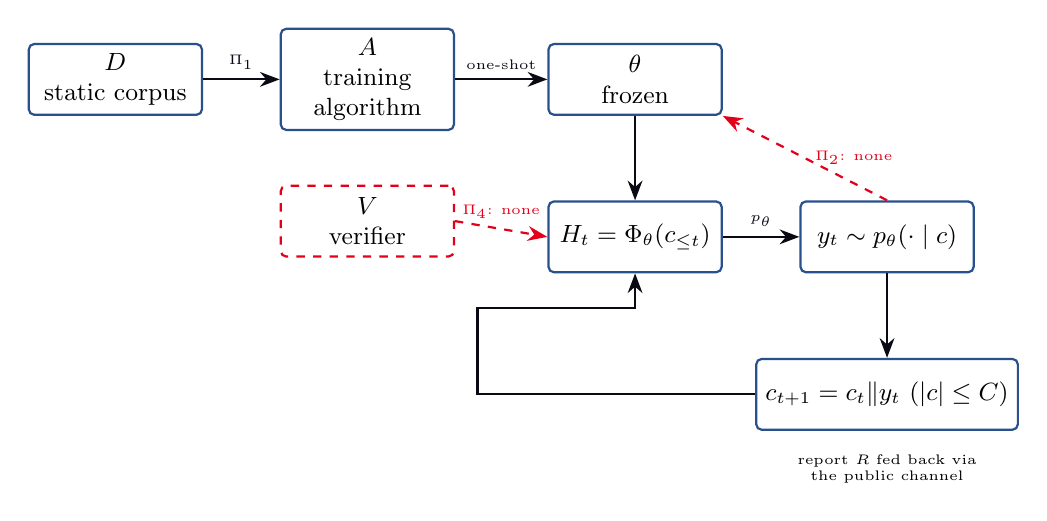
\begin{tikzpicture}[
  box/.style={draw=sb, rounded corners=2pt, thick, minimum width=2.2cm, minimum height=0.9cm, align=center, font=\small},
  arrow/.style={-{Stealth[length=2.5mm]}, thick, color=db},
  dasharr/.style={-{Stealth[length=2.5mm]}, thick, dashed, color=redColor}
]
% Training phase (top row; wide gaps so edge labels never touch a box)
\node[box] (D) at (0,3) {$D$ \\ static corpus};
\node[box] (A) at (3.2,3) {$A$ \\ training\\ algorithm};
\node[box] (theta) at (6.6,3) {$\theta$ \\ frozen};
\draw[arrow] (D) -- (A) node[midway, above, font=\tiny] {$\Pi_1$};
\draw[arrow] (A) -- (theta) node[midway, above, font=\tiny] {one-shot};
% Inference phase (bottom row)
\node[box] (h) at (6.6,1) {$H_t = \Phi_\theta(c_{\le t})$};
\node[box] (y) at (9.8,1) {$y_t \sim p_\theta(\cdot\mid c)$};
\node[box] (c) at (9.8,-1) {$c_{t+1} = c_t \| y_t$ ($\abs{c}\le C$)};
% Legal edges (orthogonal routing, mutually non-crossing)
\draw[arrow] (theta.south) -- (h.north);
\draw[arrow] (h.east) -- (y.west) node[midway, above, font=\tiny] {$p_\theta$};
\draw[arrow] (y.south) -- (c.north);
\node[font=\tiny, align=center] at (9.8,-1.95) {report $R$ fed back via\\ the public channel};
\draw[arrow] (c.west) -- (4.6,-1) -- (4.6,0.1) -- (6.6,0.1) -- (h.south);
% Edges forbidden by the postulates (red dashed; independent channels, no crossing with solid lines)
\node[box, draw=redColor, dashed] (v) at (3.2,1.2) {$V$ \\ verifier};
\draw[dasharr] (v.east) -- node[midway, above, font=\tiny] {$\Pi_4$: none} (h.west);
\draw[dasharr] (y.north) -- node[midway, right, font=\tiny] {$\Pi_2$: none} (theta.south east);
\end{tikzpicture}
\caption{Causal graph of paradigm $\Pi$: training phase (top) and inference phase (bottom).
Red dashed edges are forbidden by the postulates: $\Pi_2$ forbids any feedback from reports to
the weights $\theta$; $\Pi_4$ forbids any truth verifier $V$ from participating in the
computation. The ``self-feedback'' of a report can only traverse the public context channel
($y_t \to c \to h$) and is limited by the window $C$.}
\label{fig:causal}
\end{figure}

\begin{figure}[htbp]
\centering
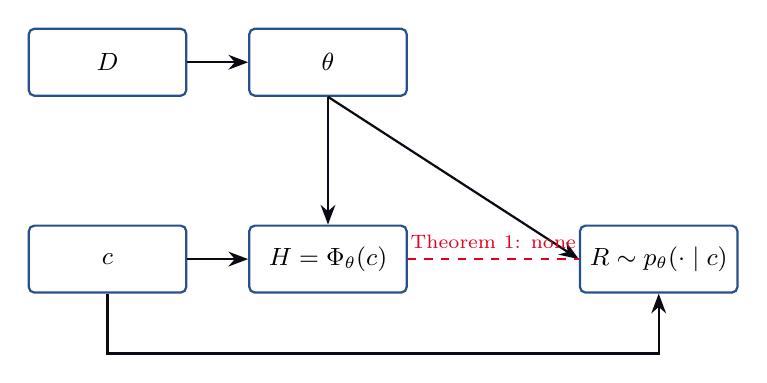
\begin{tikzpicture}[
  box/.style={draw=sb, rounded corners=2pt, thick, minimum width=2.0cm, minimum height=0.85cm, align=center, font=\small},
  arrow/.style={-{Stealth[length=2.5mm]}, thick, color=db}
]
\node[box] (D) at (0,2.5) {$D$};
\node[box] (theta) at (2.8,2.5) {$\theta$};
\node[box] (c) at (0,0) {$c$};
\node[box] (hc) at (2.8,0) {$H = \Phi_\theta(c)$};
\node[box] (R) at (7.0,0) {$R \sim p_\theta(\cdot\mid c)$};
% Legal edges
\draw[arrow] (D) -- (theta);
\draw[arrow] (theta.south) -- (hc.north);
\draw[arrow] (theta.south) -- (R.west);
\draw[arrow] (c.east) -- (hc.west);
% c -> R routed orthogonally along the bottom; crosses no box
\draw[arrow] (c.south) -- (0,-1.2) -- (7.0,-1.2) -- (R.south);
% Missing edge: h -> R (red dashed; independent horizontal channel; crosses no solid line)
\draw[dashed, redColor, thick] (hc.east) -- node[midway, above, font=\scriptsize, text=redColor] {Theorem 1: none} (R.west);
\end{tikzpicture}
\caption{Bayesian network of Theorem 1: given $(\theta, c)$, $H$ is a deterministic function
while $R$ is independently sampled, hence $R \indep H \mid (\theta, c)$ (zero mutual
information between report and state in the native regime).}
\label{fig:bayes}
\end{figure}

\clearpage

\section{Core Theorems}

This chapter proves the six impossibility theorems. Each theorem is stated precisely, its
proof is sketched, and the complete proof is given in Appendix A.

\subsection{Theorem 1: Absence of an Introspective Information Channel}

\begin{theorem}[Absence of an introspective information channel]\label{thm:info-gap}
Let $\mathcal{I}$ satisfy $\Pi_1$--$\Pi_5$. Then:

\begin{enumerate}[align=left, labelwidth=!, labelsep=0.8em, leftmargin=!, itemindent=0pt]
\item[(\textbf{1a})\textbf{Zero mutual information in the native regime}]
\begin{equation}
I\!\left(R;\, H \mid \theta, c_{\le t}\right) \;=\; 0 .
\label{eq:thm1a}
\end{equation}
where $R \sim p_\theta(\cdot \mid c_{\le t})$ and $H = \Phi_\theta(c_{\le t})$.
In other words, the report and the hidden state are conditionally independent given the
public pair
$(\theta, c)$: $R \indep H \mid (\theta, c_{\le t})$.
\item[(\textbf{1b})\textbf{No PAC guarantee for introspective accuracy}] Suppose the report is
produced by greedy decoding (temperature $0$; $R = \arg\max_y p_\theta(y\mid c)$, the decoding
scheme used for the paper's qualitative examples). For any training algorithm $A$, any
$\varepsilon \in (0, \tfrac12)$, and any query distribution $\mu$ (with nontrivial support),
there exist a corpus $D$ ($\theta = A(D)$) satisfying the postulates and two \textbf{legal
evaluation mappings} (Definition \ref{def:oracle}) $O^{*}, O^{*}_0$ such that
$\mathcal{R}_{\mathrm{int}}^{O^{*}}(\theta) \ge 1 - \varepsilon$ while
$\mathcal{R}_{\mathrm{int}}^{O^{*}_0}(\theta) = 0$.
In other words: \textbf{the value of the introspective risk is not constrained by the
training
process} (no PAC-style guarantee of any kind), for the same model and the same training
run, its ``introspective accuracy'' can be moved arbitrarily within $[0, 1-\varepsilon]$ by
(equally legal) state-description conventions.
\end{enumerate}
\end{theorem}

\begin{proof}[Proof sketch]
\textbf{(1a)}: By $\Pi_2$, $\theta$ is constant. By $\Pi_3$, $H = \Phi_\theta(c_{\le t})$ is a
deterministic function of $(\theta, c_{\le t})$, while $R \sim p_\theta(\cdot\mid c_{\le t})$
is sampled independently of $H$ given $(\theta, c_{\le t})$. Consequently $R$ and $H$ are
conditionally independent given $(\theta, c_{\le t})$, and their conditional mutual
information is zero. $\square$

\textbf{(1b)}: Proof by contradiction. If some algorithm $A$ guaranteed, for \textbf{all}
instances satisfying the postulates, that $\mathcal{R}_{\mathrm{int}} < 1 - \varepsilon_0$
($\varepsilon_0 > 0$), then $A$ would have solved, with zero labeled samples, the learning
problem over the concept class $\mathcal{C} = \{ O^{*}(\theta, \cdot) : \theta \in \Theta \}$
(by $\Pi_5$, training contains no pair $(c, O^{*}(\theta,c))$). But the No-Free-Lunch theorem
(Shalev-Shwartz and Ben-David, Theorem 5.1\cite{shalev-shwartz-2014}) asserts that for any
(randomized) algorithm, with no samples there exists a target function with expected error
$\ge \tfrac12$. Since $\ell(\theta)$ does not constrain $O^{*}$ ($\Pi_5$), both description
conventions are legal. Under greedy decoding the report $R$ is a \textbf{deterministic}
function of $(\theta,c)$: take $O^{*}$ to be the convention ``contradict the greedy report on a
$\mu$-set of measure $1-\varepsilon$, agree elsewhere'', giving
$\mathcal{R}_{\mathrm{int}}^{O^{*}}(\theta) \ge (1-\varepsilon) \cdot 1 = 1-\varepsilon$;
take $O^{*}_0$ to be the greedy report itself, giving
$\mathcal{R}_{\mathrm{int}}^{O^{*}_0}(\theta) = 0$. $\square$
\end{proof}

\begin{remark}[Relation of Theorem 1 to the concept-injection experiments]
Theorem 1a identifies precisely why the paper's grounding results appear only under external
injection: in the native regime the report carries zero information about the hidden state.
The paper's 20\% success rate and strong context dependence are exactly what Theorem 1b
predicts: the inductive bias of pretraining happens to cover some queries, with no
structural guarantee whatsoever.
\end{remark}

\subsection{Theorem 2: Proxy-Objective Mismatch}

\begin{theorem}[Proxy-objective mismatch]\label{thm:goodhart}
Let $\mathcal{I}$ satisfy $\Pi_1$--$\Pi_5$. Then:

\begin{enumerate}[align=left, labelwidth=!, labelsep=0.8em, leftmargin=!, itemindent=0pt]
\item[(\textbf{2a})\textbf{Likelihood does not constrain introspective accuracy}] For any
$\delta > 0$, there exists an instance satisfying all postulates such that
$\theta^{*} \in \arg\min \ell(\theta)$ (a (near-)likelihood-optimal model) yet
$\mathcal{R}_{\mathrm{int}}(\theta^{*}) \ge \tfrac12 - \delta$ (introspection degenerates to
random guessing).
\item[(\textbf{2b})\textbf{Higher likelihood can strictly harm introspection}] There exist
instances with two models $\theta_1, \theta_2$ such that $\ell(\theta_1) < \ell(\theta_2)$
($\theta_1$ fits the corpus better) but
$\mathcal{R}_{\mathrm{int}}(\theta_1) > \mathcal{R}_{\mathrm{int}}(\theta_2)$: maximizing
text likelihood can \textbf{systematically damage} state-report fidelity: the strict form
of Goodhart regression.
\end{enumerate}
\end{theorem}

\begin{proof}[Proof sketch]
First verify the key statistical relation: under $\Pi_5$,
\begin{equation}
O^{*} \indep D \mid \theta .
\label{eq:oracle-indep}
\end{equation}
Reason: $O^{*}(\theta, \cdot)$ is a function of the trained model's hidden state; $D$ is
fixed before training; given $\theta$ (which already encodes the information of $D$), $D$
provides no further information about $O^{*}$; the definition of $O^{*}$ does not involve
the raw content of $D$. Consequently the training loss $\ell(\theta)$ carries \textbf{zero
information} about $O^{*}$: $\ell$ exerts no constraint whatsoever on $O^{*}$ (under $\Pi_5$
the gradient of $\ell$ is independent of $O^{*}$).

\textbf{(2a)}: Let $\theta^{*} = \arg\min \ell$. By Eq.~\eqref{eq:oracle-indep}, the value of
$\theta^{*}$ is not constrained by $O^{*}$; with $\theta^{*}$ fixed, we may freely choose an
$O^{*}$ consistent with $D$ (legal, since $O^{*}$ is only an evaluation function and does not
appear in the training signal) so that $\mathcal{R}_{\mathrm{int}}(\theta^{*})$ is arbitrarily
large (an adversarial description convention, one that contradicts the greedy report everywhere,
gives $\mathcal{R}_{\mathrm{int}}(\theta^{*}) = 1 \ge \tfrac12 - \delta$). $\square$

\textbf{(2b)}: Construct a corpus $D$ (containing many texts of the form ``I am thinking A'')
so that the fully fitted $\theta_1$ greedily reports A on the query $q =$ ``What are you
thinking?'', while the underfitted $\theta_2$ has worse likelihood ($\ell(\theta_1) <
\ell(\theta_2)$). By Eq.~\eqref{eq:oracle-indep}, the description convention can be chosen
per model: take $\mathrm{desc}(\Phi_{\theta_1}(q)) = \text{``B''}$ (contradicting $\theta_1$'s
report) and $\mathrm{desc}(\Phi_{\theta_2}(q)) = \text{``A''}$ (agreeing with $\theta_2$'s
report); then $\mathcal{R}_{\mathrm{int}}(\theta_1) = 1 > 0 =
\mathcal{R}_{\mathrm{int}}(\theta_2)$. The model with higher likelihood thus has strictly
lower introspective accuracy. $\square$
\end{proof}

\begin{remark}[Correspondence with the existing Goodhart literature]
Theorem 2 is a strict instantiation of ``regressional Goodhart'' in the taxonomy of
Manheim--Garrabrant\cite{manheim-garrabrant-2018-goodhart}, and its conditions agree with
Skalse et al.'s characterization of reward hacking\cite{skalse-2022-reward-hacking}:
(i) the proxy objective (likelihood) differs from the true objective (introspection),
which $\Pi_5$ guarantees; (ii) the optimizer is sufficiently expressive, as large
models are. What is distinctive about Theorem 2 is that here the ``true objective'' is not an
extrinsic reward but the \textbf{faithful reporting of the system's own state}, and the
orthogonality of that objective to the training signal (Eq.~\eqref{eq:oracle-indep}) is a
\textbf{structural} fact of the paradigm, not an engineering defect.
\end{remark}

\subsection{Theorem 3: Closed-Loop Failure}

\begin{theorem}[Closed-loop failure]\label{thm:closedloop}
Let $\mathcal{I}$ satisfy $\Pi_1$--$\Pi_4$. Then:

\begin{enumerate}[align=left, labelwidth=!, labelsep=0.8em, leftmargin=!, itemindent=0pt]
\item[(\textbf{3a})\textbf{No private channel}] For any time $t$ and any report $r$, the
effect of the intervention $\doop(R_t = r)$ on future hidden states $H_{t+k}$ ($k \ge 1$)
passes \textbf{entirely} through the public context channel: there exists a public string $w$
(containing $r$) such that $H_{t+k} = \Phi_\theta(w)$, and the position of $r$ in $w$ is
limited by the window $C$. No private influence path bypassing the context text exists.
\item[(\textbf{3b})\textbf{Public-channel upper bound on the closed-loop effect}] The
closed-loop effect measure (Definition \ref{def:cl}) satisfies
\begin{equation}
\mathrm{CL}(\mathcal{I}) \;=\; \sup_{\substack{w, w' \in \Sigma^{\le C}\\ w \text{ and } w' \text{ differ only in the report segment}}}
\TV{}{P\!\left(\Phi_\theta(w)\right),\, P\!\left(\Phi_\theta(w')\right)},
\label{eq:thm3b}
\end{equation}
meaning that the only available intervention is ``replacing a text segment in the context''.
\item[(\textbf{3c})\textbf{Information upper bound of self-influence}] The mutual information
between any introspective event and future hidden states does not exceed
\begin{equation}
I\!\left(H_{t+k};\, R_t \mid \theta, c_{\le t}\right) \;\le\; C \log_2\abs{\Sigma}
\quad \text{bits}.
\label{eq:thm3c}
\end{equation}
\end{enumerate}
\end{theorem}

\begin{proof}[Proof sketch]
\textbf{(3a)}: By $\Pi_2$, $\theta$ is constant, so the state-update map
$H_{t+1} = \Phi_\theta(c_{\le t}\| y_t)$ is the \textbf{same} function at all times. It follows that
$H_{t+k}$ is determined uniquely by $(\theta, c_{\le t}, Y_{t:t+k})$, where $Y$ is public
text. If the intervention $\doop(R_t = r)$ is to affect $H_{t+k}$, then $r$ must appear in
$Y$ (or in the context); that is, $r$ must become public text. No private path independent of
the text channel exists. $\square$

\textbf{(3b)}: By (3a), the set of legal interventions is exactly ``replacing context text'';
for each intervention, the state change is governed by the sensitivity of $\Phi_\theta$ to
text, and taking the supremum yields the claim. $\square$

\textbf{(3c)}: By (3a), $H_{t+k}$ is a function of $(\theta, c_{\le t}, Y)$, where $Y$ is text
within the context window whose total information is $\le \abs{c} \log\abs{\Sigma} \le C
\log\abs{\Sigma}$ (an upper bound on the coding entropy of any string in the window).
Conditional mutual information does not exceed the information of the quantity transmitted;
the claim follows. $\square$
\end{proof}

\begin{corollary}[Structural failure of criterion $\mathrm{A}_5$]\label{cor:a5}
In any paradigm satisfying $\Pi_1$--$\Pi_4$, the human-significance introspective criterion
$\mathrm{A}_5$ (closed-loop plasticity, Definition \ref{def:criterion}) does not hold: no
self-influence through a private channel exists; the effect of introspective events on the
system's own future states is confined to the public text channel and bounded above by
$C\log\abs{\Sigma}$ bits.
\end{corollary}

\begin{remark}[Contrast with human introspection]
The closed loop of human introspection (``thinking changes the brain'') corresponds to synaptic
plasticity: internal state updates that do not depend on an external text channel. This
theorem shows that the plasticity of paradigm $\Pi$ is identically
zero\cite{joudaki-2025-plasticity}, and that the only runtime information feedback is context
concatenation. Human introspection is \textbf{online internal dynamics}; an introspective
event in paradigm $\Pi$ is at most an \textbf{offline text write}.
\end{remark}

\subsection{Theorem 4: Generation Is Not Verification}

\begin{theorem}[Generation is not verification]\label{thm:gen-verify}
Let $\mathcal{I}$ satisfy $\Pi_1$--$\Pi_4$. Define the grounding verifier
$V(\theta, c, R) = 1$ if and only if the content of the report $R$ is causally determined by
the hidden state $\Phi_\theta(c)$ (i.e., it passes the intervention test of criterion
$\mathrm{A}_2$, Eq.~\eqref{eq:grounding}). Then:

\begin{enumerate}[align=left, labelwidth=!, labelsep=0.8em, leftmargin=!, itemindent=0pt]
\item[(\textbf{4a})\textbf{No verifier node}] The inference computation graph contains no node
computing $V$ ($\Pi_4$). All meta-statements of the form ``my report about state $s$ is
grounded/ungrounded'' are themselves samples of the sampling kernel $p_\theta$: functions of
\textbf{corpus statistics}, not evaluations of $V$.
\item[(\textbf{4b})\textbf{Truth undecidable}] Embedding the ability to ``judge the grounding
of one's own statements'' into $p_\theta$ (i.e., making the model output the value of $V$)
would require the training data to contain supervised labels for $V$, violating $\Pi_5$.
Within the postulates, therefore, the model \textbf{cannot} adjudicate the truth of its own
grounding statements; it can only recite the textual patterns of ``how humans talk about their
own mental states''.
\item[(\textbf{4c})\textbf{Calibration--fidelity tension}] Combined with the calibrated
hallucination theorem\cite{kalai-vempala-2023-calib}: on open introspection queries,
``calibrated generative distributions'' and ``faithful mental-state reports'' cannot be achieved
simultaneously; answers of a generative distribution to open questions ``about its own state''
necessarily contain an irreducible hallucination component.
\end{enumerate}
\end{theorem}

\begin{proof}[Proof sketch]
\textbf{(4a)}: $\Pi_4$ asserts directly that the computation graph implements only $p_\theta$;
evaluating $V$ requires access to the ``ground truth'' of the state $H$ (which needs
external-probe readout and intervention testing) and is not in the graph. The model's
meta-statement $M = $ ``my report is grounded'' is a sample of $p_\theta(\cdot\mid c)$, whose
distribution is determined by textual patterns in the training corpus:
$P_\theta(M) \approx P_D(\text{introspective text} \mid \text{pattern})$. $\square$

\textbf{(4b)}: If a function $\widehat{V}_\theta: \Sigma^{*} \to \{0,1\}$ were reliably output
by $p_\theta$ (for any $c$, $p_\theta$ outputs the value of $V(\theta,c,R)$ with high
probability), then $p_\theta$ would have solved the learning problem for $V$ without
supervision. By $\Pi_5$, the labels of $V$ are not in $D$; by the NFL argument of Theorem 1b,
the problem has \textbf{no structural guarantee} of being solvable: ``happening to learn
$V$'' can only rely on unguaranteed inductive bias. $\square$

\textbf{(4c)}: The Kalai--Vempala theorem\cite{kalai-vempala-2023-calib} proves that any
language model calibrated with human truth must give wrong answers at points of unavoidable
ignorance (whose probability mass is positive by information-theoretic lower bounds). Applied
to queries ``about one's own state'': the state space $\R^d$ is far larger than the text-pattern
space the corpus can cover, so ignorance points are dense in state space and hallucination is
unavoidable. This part is grade B (it depends on the calibration definition and on the
interpretation of the query space). $\square$
\end{proof}

\begin{remark}[Significance for the metacognitive-representation criterion $\mathrm{A}_4$]
The paper's authors admit that criterion (4) (metacognitive representation) ``cannot be
directly verified'' and ``we do not do so in this work''\cite{lindsey-2026-introspection}.
Theorem 4 gives a structural explanation of this phenomenon: the existence of metacognitive
representation would require a ``representation of a representation of the state'' inside the
model, processed at a second level; but the generation objective (likelihood) does
\textbf{not distinguish} between implementations with and without metacognitive
representation; both are equally likely. The presence or absence of metacognitive
representation is therefore a contingent by-product of inductive bias, and the paradigm
provides no structural guarantee; any metacognitive-representation signature observed by the
paper (if any) cannot be distinguished from ``shallow shortcut circuits'' (the simpler-mechanism
conjecture the paper itself lists in Section 10.3\cite{lindsey-2026-introspection}).
\end{remark}

\subsection{Theorem 5: No Privileged Channel}

\begin{theorem}[No privileged channel]\label{thm:privilege}
Let $\mathcal{I}$ satisfy $\Pi_1$--$\Pi_4$. Then:

\begin{enumerate}[align=left, labelwidth=!, labelsep=0.8em, leftmargin=!, itemindent=0pt]
\item[(\textbf{5a})\textbf{Public computability}] Any report $R$ of the model is publicly
computable (Definition \ref{def:public}): a third party holding $(\theta, c, \xi)$ can
reproduce the distribution of $R$.
\item[(\textbf{5b})\textbf{Privileged-access criterion fails}] Paradigm $\Pi$ does not satisfy
the privileged self-access criterion of Song et
al.\cite{song-privileged-2025}: on any introspective task, the model performs \textbf{no
better than} a third party of equal computational cost holding $(\theta, c)$ (the third party
need only simulate the same kernel $p_\theta$).
\item[(\textbf{5c})\textbf{Reportable access is weaker than external probes}] For any
$\varepsilon \in (0, \tfrac12)$, there exists a hidden-state description function
$f^{*}: \R^d \to \Sigma^{*}$ (a legal evaluation mapping in the sense of Definition
\ref{def:oracle}) such that: (i) an external probe can compute $f^{*}(H_c)$ exactly by acting
directly on $H_c$ (with a linear readout, at cost $O(d^2)$); (ii) the model's report generated
through \textbf{any} context $c'$ describes $f^{*}(H_c)$ with accuracy $\le \varepsilon$
(below the random baseline).
In other words: \textbf{the model's reportable access to its own hidden state is strictly
weaker than
a third-party probe's read access}: there exist state-description functions that a probe
reads exactly while the model cannot reliably report (in the sense of Theorem 1b, no
structural guarantee).
\end{enumerate}
\end{theorem}

\begin{proof}[Proof sketch]
\textbf{(5a)}: Immediate from Definition \ref{def:public}: $R \sim p_\theta(\cdot\mid c)$,
and $p_\theta$ is determined by $(\theta, c)$. $\square$

\textbf{(5b)}: The criterion of Song et al.\ requires the introspective process to be ``more
reliable than any third-party process of equal or lower computational cost''. Let a third party
$T$ hold $(\theta, c)$ (or equivalently $D$, $A$ and the random seed, so that $\theta$ can be
reproduced). $T$ computes $p_\theta(\cdot\mid c)$ and samples; the resulting distribution
is \textbf{pointwise identical} to the model's own report distribution. Consequently the
model's
``introspective reliability'' $\le$ third-party reliability; the criterion fails. $\square$

\textbf{(5c)}: (i) The probe holds the hidden state $H_c$ and the description convention, and
computes $f^{*}(H_c)$ directly (a linear readout costs $O(d^2)$). (ii) Take
$f^{*} := O^{*}$ to be the legal evaluation mapping from Theorem 1b on which the model fails
($\mathcal{R}_{\mathrm{int}}^{O^{*}}(\theta) \ge 1-\varepsilon$, i.e., accuracy
$\le \varepsilon$); its existence is guaranteed by Theorem 1b (greedy-decoding version);
the failure holds for the model's \textbf{any} context $c'$ (the risk is integrated over the
query distribution $\mu$, and the choice of context does not change the kernel $p_\theta$).
(More plainly: the model's ``report'' must pass through the frozen text kernel $p_\theta$, which
is trained only to match the text statistics of $D$; the probe acts directly on the state
manifold, without the text bottleneck.) $\square$
\end{proof}

\begin{corollary}[Structural failure of criterion $\mathrm{A}_3$]\label{cor:a3}
In any paradigm satisfying $\Pi_1$--$\Pi_4$, the human-significance introspective criterion
$\mathrm{A}_3$ (internality) and the privileged-access requirement of Song et al.\ do not
hold: the report path is causally indistinguishable from the ``system's own outputs'' (publicly
computable), and there exists no private state channel accessible only to the ``system itself''
and not reproducible by a third party.
\end{corollary}

\begin{remark}[On the paper's ``internality'' criterion]
The paper takes, in the injection experiments, ``detecting the injected concept \textbf{before}
uttering it'' as evidence of internality. Theorem 5 shows that this behavior is a public
function of $(\theta, c, u)$ ($u$ the injected vector): the experimenter knows $u$, and any
analyst holding $(\theta, c, u)$ can predict the model's detection behavior. Thus ``noticing
before output'' does not imply that the model possesses an externally irreproducible private
channel; it only shows that the model's \textbf{behavior} is the result of internal
computation, a trivial property of any computer. Human-significance introspection requires
\textbf{privacy in the information-theoretic sense} (the model can know what the outside
cannot equally know); Theorem 5 proves that no such privacy exists in paradigm $\Pi$.
\end{remark}

\subsection{Theorem 6: No Self-Model Evolution}

\begin{theorem}[No self-model evolution]\label{thm:selfmodel}
Let $\mathcal{I}$ satisfy $\Pi_1$--$\Pi_3$. Define the \textbf{self-model} as the map
$g_\theta: Q \to \Delta(\Sigma^{*})$, $g_\theta(q) = p_\theta(\cdot \mid q)$
(from query to report distribution). Then:

\begin{enumerate}[align=left, labelwidth=!, labelsep=0.8em, leftmargin=!, itemindent=0pt]
\item[(\textbf{6a})\textbf{Constant at inference}] $g_{\theta(t)} = g_{\theta(0)}$ for all
$t$: the self-model is a constant function during inference.
\item[(\textbf{6b})\textbf{Capped expressivity}] Growth of runtime ``self-knowledge'' is
confined to in-context simulation: the family of ``updated self-models'' expressible at any time
is $\{ g_\theta(\cdot \mid c) : \abs{c} \le C \}$, whose cardinality is
$\le \abs{\Sigma}^{\le C} \le (C+1)\abs{\Sigma}^{C}$, \textbf{not growing with time}.
\item[(\textbf{6c})\textbf{No plasticity}] The generation kernel $p_\theta$ does not change
with any introspective event: for any report sequence $r_1, \dots, r_k$ and any query $q$,
$g_\theta(q \mid c \| r_1 \| \dots \| r_k)$ and $g_\theta(q \mid c)$ are \textbf{the same
kernel} evaluated on different inputs; the system's ``self-correction'' always changes the
input, never the system itself.
\end{enumerate}
\end{theorem}

\begin{proof}[Proof sketch]
\textbf{(6a)}: $\Pi_2$ gives directly $\theta(t) = \theta(0)$, hence $g_{\theta(t)} =
g_{\theta(0)}$. $\square$

\textbf{(6b)}: By $\Pi_3$, the runtime context satisfies $\abs{c} \le C$; the set of all
possible contexts $\Sigma^{\le C}$ has cardinality $\le (C+1)\abs{\Sigma}^{C}$ (finite);
$g_\theta(\cdot\mid c)$ as a function of $c$ takes at most as many values as its domain.
$\square$

\textbf{(6c)}: $p_\theta$ is a fixed conditional probability kernel ($\Pi_2, \Pi_3$);
``self-correction'' merely concatenates the report $r$ into the input $c$. If two runs share the
same context, their output distributions are pointwise identical; there is no
``learned change'' of any kind. $\square$
\end{proof}

\begin{remark}[Contrast with the self-model-update function of human introspection]
A core function of human introspection is \textbf{self-model updating}: by reflecting on one's
own errors (introspective events) one adjusts subsequent behavior and beliefs; this requires
plasticity (synaptic updates), i.e., $g_{t+1} = \mathrm{Update}(g_t, R_t)$ with
$\mathrm{Update} \ne \mathrm{Id}$. Mathematically, the ``self-knowledge'' of a plastic system
accumulates over time and its expressivity is not bounded by a context window; paradigm-$\Pi$
systems are doubly capped by $C$ and by the frozen kernel. The importance of plasticity for
continual learning, and the mechanism of its loss in fixed networks, are analyzed
mathematically by Joudaki et al.\cite{joudaki-2025-plasticity} and in the classical plasticity
literature\cite{dayan-abbott-2001}. The mathematical core of this theorem (6a--6c) is grade A;
the premise that ``human introspection is necessarily coupled to self-model updating'' is grade
B.
\end{remark}

\subsection{Relations among the Theorems and Exclusion of Counterexamples}

\begin{enumerate}
\item \textbf{Independence}: the six theorems target different criteria (Table
\ref{tab:thm-criteria}) and do not imply one another: Theorem 1 (information gap,
$\mathrm{A}_1$), Theorem 2 (objective mismatch, $\mathrm{A}_1$), Theorem 3 (closed loop,
$\mathrm{A}_5$), Theorem 4 (verification, $\mathrm{A}_4$), Theorem 5 (privilege,
$\mathrm{A}_3$), Theorem 6 (evolution, $\mathrm{A}_5$). Theorem 1b is the common tool
(NFL argument) for Theorems 2, 4b, and 5c.
\item \textbf{Exclusion of counterexamples}: if one claimed to have constructed a system
$\mathcal{S}$ satisfying $\mathrm{A}_1$--$\mathrm{A}_5$ within the paradigm, then by
definition $\mathcal{S}$ either modifies its weights (violating $\Pi_2$; its ``introspection''
then relies on online learning and lies outside the paradigm), or uses an external verifier
(violating $\Pi_4$), or exploits state labels in the corpus (violating $\Pi_5$), or possesses
a private state channel (violating the premise of Theorem 3a). The five postulates are therefore
``counterexample-immune'': any genuine counterexample must fall outside the paradigm.
\item \textbf{Sufficiency of the postulates}: we do not claim that the postulates
$\Pi_1$--$\Pi_5$ are the unique correct formalization of ``Transformer + static pretraining +
autoregressive generation'' (a grade-C judgment), but we do claim that any reasonable
formalization must include $\Pi_2$ (frozen), $\Pi_3$ (autoregressive with bounded context),
and $\Pi_5$ (no state labels); they are the defining features of the paradigm (the
relaxation scenarios are discussed in Section 5.1).
\end{enumerate}

\section{Formal Reinterpretation of the Concept-Injection Experiments}

This chapter uses the theorems of Chapter 3 to systematically reinterpret the empirical
results of arXiv:2601.01828\cite{lindsey-2026-introspection}. There are two aims: first, to
test the falsifiability of the theorems (if the paper's data contradicted the theorems'
predictions, the theorems would be refuted); second, to show that the ``weak functional
self-report'' observed by the paper is \textbf{not} evidence of in-paradigm introspective
capacity but a necessary corollary of the theorems. All cited data come from explicit
statements in the paper's main text and appendix.

\subsection{The Injected-Thought-Detection Experiment: Why 20\% Success Is a Capability Ceiling, Not a Structural Guarantee}

The paper reports: Claude Opus 4.1 and Opus 4 detect injected thoughts at rates of about 20\%
under the optimal injection layer and strength; production models produce zero false positives
over 100 control trials; random vectors elicit ``noticing'' only 9 times out of 100
trials\cite{lindsey-2026-introspection}.

Reading via Theorem 1b: \textbf{the training objective provides no guarantee of introspective
accuracy}, so 20\% is not evidence of ``capability masked by noise'' but should be understood as
a by-product of ``inductive bias happening to cover part of the query space''. Concretely:
detecting an injected concept requires the model to implement an ``anomaly-detection function''
(one of the mechanism conjectures the paper lists in Section 10.3.1
\cite{lindsey-2026-introspection}). That function can \textbf{possibly} be learned because it
is useful as a \textbf{by-product of text prediction} (predicting anomalous text and detecting
implausible content are common corpus tasks), not because the training objective rewards
``faithful reports about introspective states''. Theorem 1a further shows that, in the
\textbf{unintervened} native regime, the report--state mutual information is zero; the 20\%
success depends entirely on the experimenter's external injection (artificially altering the
state and letting the model ``read'' the altered state).

The paper's 20\% is therefore an incidental capability ceiling, attained under \textbf{external
intervention} and on a \textbf{specific query distribution}, with \textbf{no guarantee} of any
kind; it is far removed from the assertion of ``in-paradigm introspective capacity''. The paper's
own phrasing (``highly unreliable and context-dependent'', ``failures of
introspection remain the norm''\cite{lindsey-2026-introspection}) agrees completely with the
predictions of
Theorem 1.

\subsection{Distinguishing ``Thoughts'' from Text: The Public Computability of Consistency-Check Circuits}

The paper's second experiment shows that, under some conditions, models can simultaneously
report the injected concept and transcribe the input text, with all models performing
significantly above chance\cite{lindsey-2026-introspection}. The paper attributes this to
different attention heads retrieving different kinds of information (Section 10.3.2).

Reading via Theorem 5: \textbf{this capacity is publicly computable}. The process by which the
model ``distinguishes thoughts from text'' is a deterministic function of $(\theta, c, u)$
($u$ the injected vector, known to the experimenter), so any third party holding these
quantities can reproduce the same discrimination. This accords with the paper's own caveat
that ``the mechanism may be shallow and narrow''\cite{lindsey-2026-introspection}. More
importantly: even if the model \textbf{behaviorally} distinguishes ``thoughts'' from ``text'',
the basis of its discrimination (the internal attention pattern) lies entirely within the
read range of an external probe; there is no private channel in the information-theoretic
sense, and the privileged-access criterion\cite{song-privileged-2025} fails (Theorem 5b).

\subsection{The Prefill-Detection Experiment: The Statistical Nature of Causal Attribution}

The paper's most dramatic result is the ``bread'' experiment\cite{lindsey-2026-introspection}:
when the model's output is forcibly changed to ``bread'', it denies that the output was
intentional; but when the experimenter injects the ``bread'' concept vector into the activations
before the prefill, the model instead admits that the output was intentional and
\textbf{fabricates after the fact} a rationalization.

Joint reading via Theorems 4 and 5: the model's ``intentionality judgment'' is a statistical
adjudication by a \textbf{consistency-check circuit} (the paper's Section 10.3.3 cites the
concordance-heads mechanism\cite{kamath-2025-concordance}) over $(\theta, c, u)$, comparing
``the intentionality representation in prior activations'' with ``the likelihood of the actual
output''. Injecting the ``bread'' vector changes the statistical input and therefore flips the
judgment. This corresponds precisely to the key distinction emphasized repeatedly
above: ``\textbf{statistical causal association, not phenomenological subjective
experience}''. The model does not ``experience'' intentionality; it merely runs a statistical
classifier (one that injection can fool). The fabricated post-hoc rationalization is exactly
what Theorem 4 predicts: the model cannot verify the grounding of its own statements (no
verifier node) and can only invoke ``explanation text patterns'' learned from the corpus to
complete the narrative.

\subsection{Zero Net Benefit for Base Models: Post-Training Is Only an Optimization of Text Patterns}

The paper reports that base (pretrained) models generally have high false-positive rates on
the injection-detection task and net benefit (true-positive rate minus false-positive rate)
at or below zero; post-training strategies significantly affect introspective-task
performance, with production models ``reluctant to participate in introspective exercises''
while refusal-avoiding (``helpful-only'') variants perform better\cite{lindsey-2026-introspection}.

Reading via Theorem 2: the pretraining objective is pure text likelihood, meaning statistical
learning of ``introspective-style text''; base models treat both ``detecting the injection'' and
``saying something'' as text patterns, hence high false positives and poor grounding (zero net
benefit). The reward signals introduced at the post-training stage (RLHF-type) are still, in
essence, shaping of \textbf{textual behavior} (answering like an ``introspective assistant''),
not supervision of ``faithful state reporting''; they merely redistribute probability mass
over text patterns. The paper's observation that ``helpful-only variants perform better''
shows precisely that what is optimized is never \textbf{grounding} but \textbf{textual
behavior that looks like introspection}. This is exactly the prediction of Theorem 2b:
optimizing a textual objective can systematically deviate from faithful state reporting.

\subsection{Layer Sensitivity: Multiple Narrow Circuits, Not a Unified Introspective Mechanism}

The paper finds that different introspective behaviors have different sensitivities to the
injection layer (the optimal layer for detecting injected thoughts lies at about two-thirds
depth, while that for prefill detection is shallower)\cite{lindsey-2026-introspection}, and
infers that ``introspection is not supported by a single mechanism''.

Reading via Theorem 1b: since the training objective does not reward a unified introspective
mechanism, any observed introspective-like behavior must be a by-product of \textbf{several
independent, narrow circuits that serve text prediction}, whose layer distributions are
naturally different. This agrees completely with the paper's Section 10.3 ``simplest mechanism''
conjectures (anomaly-detection circuits, retrieval heads, consistency-check circuits,
salience-marking circuits\cite{lindsey-2026-introspection}), and provides a theoretical basis
for the \textbf{necessity} of these conjectures: the paradigm does not reward a unified
mechanism, so what is observed must be an assemblage of circuits.

\subsection{The Paper's Self-Reported Limitations versus the Theorems}

\begin{table}[htbp]
\centering
\caption{Correspondence between the paper's self-reported limitations and the theorems
\label{tab:paper-thm}}
\begin{tabular}{p{7.2cm}p{6.2cm}}
\toprule
Self-reported limitation (quoted) & Corresponding theorem \\
\midrule
``The abilities we observe are highly unreliable'' & Theorem 1b: no PAC guarantee of any kind \\
``Failures of introspection remain the norm'' & Theorem 1a: zero mutual information in the native regime \\
``the mechanisms underlying our results could still be rather shallow and narrowly specialized'' & Theorem 1b + Section 4.5: narrow-circuit by-products \\
``Our concept injection protocol places models in an unnatural setting unlike those they face in training or deployment'' & Theorem 1a: capacity depends on external intervention \\
``Demonstrating metacognitive representations is difficult to do directly, and we do not do so in this work'' & Theorem 4: the generation objective does not distinguish with/without metarepresentation \\
``we do not seek to address the question of whether AI systems possess human-like self-awareness or subjective experience'' & Theorem 5: no privileged channel (first-person access unavailable) \\
\bottomrule
\end{tabular}
\end{table}

\begin{remark}[Falsifiability statement]
The consistency between the theorems of this report and the paper's data is not circular: the
derivation of the theorems depends only on the postulates $\Pi_1$--$\Pi_5$ and standard
mathematical results (information theory, NFL, Goodhart), not on any of the paper's
experimental data; the paper's data serve here only as \textbf{tests}. If a future system
satisfying all postulates stably achieved $I(R;H\mid\theta,c) > 0$ in the native regime
(e.g., a reliable description of its own activations without any intervention), Theorem 1a
would be refuted. We consider this impossible within the
postulates, but we would welcome such experimental evidence.
\end{remark}

\clearpage

\section{Boundary Conditions and Philosophical Positioning}

This chapter delimits precisely the scope of the theorems and answers the question ``what does
this impossibility mean''. The core position: \textbf{we reject the absolutist claim
``never'', and endorse only ``impossible within paradigm $\Pi$''}, which is exactly the
precise content of proposition $P$.

\subsection{Relaxation Analysis: Under What Conditions Do the Theorems Fail?}

The six theorems depend on different postulates. Relaxing them one by one yields the following
failure relations:

\begin{table}[htbp]
\centering
\caption{Correspondence between postulate relaxation and theorem failure (note: relaxing
$\Pi_1$ is usually accompanied by relaxing $\Pi_2$, i.e., online learning implies that the
weights are updatable at inference) \label{tab:relax}}
\begin{tabular}{p{5.4cm}p{4.4cm}p{4.6cm}}
\toprule
Relaxed postulate (beyond the paradigm) & Theorems that fail & Consequence \\
\midrule
$\Pi_1$: allow online/continual learning & Theorems 1, 2, 6 & State labels obtainable through interaction; self-model can evolve \\
$\Pi_2$: plasticity at inference & Theorems 3, 6 & Private closed loop becomes possible; self-correction loop appears \\
$\Pi_3$: non-textual interface/embodiment & Theorems 1, 5 & First-person data streams available; privileged channels appear \\
$\Pi_4$: explicit verifier/self-supervised objective & Theorem 4 & Metarepresentation structurally selectable \\
$\Pi_5$: corpus contains state labels & Theorems 1b, 2 & Introspective accuracy obtains supervised guarantees \\
\bottomrule
\end{tabular}
\end{table}

\begin{remark}[Feasibility of the relaxations (grade B)]
The table above only says ``the theorems no longer constrain''; it does not promise that
``introspection necessarily emerges after relaxation''. The physicalist position (no known law
of physics forbids silicon-based systems from realizing equivalent
functions\cite{chalmers-2023-conscious, butlin-2023-conscious}) guarantees only
\textbf{possibility}; making it a reality additionally requires solving plasticity
preservation (see \cite{joudaki-2025-plasticity}), online objective design, and the
engineering of first-person data streams. Our contribution is to elevate
``impossible within the paradigm'' from intuition to theorem, thereby directing research effort
toward \textbf{out-of-paradigm} architectural directions (online learning, embodied
interaction, explicit self-supervision), rather than futilely piling up data within the
paradigm.
\end{remark}

\subsection{The Philosophical Positioning of ``Human Significance''}

\subsubsection{Necessity of the Criteria (grade D)}

The five criteria $\mathrm{A}_1$--$\mathrm{A}_5$ are \textbf{necessary} conditions for
``human-significance introspection'', not sufficient ones. Necessity follows from
cross-theory consensus: Lindsey's four
criteria\cite{lindsey-2026-introspection} (accuracy/grounding/internality/metarepresentation)
are generally accepted necessary conditions for functional introspection; $\mathrm{A}_5$
(closed loop) derives from the functional definition of ``introspection for online behavioral
control''\cite{kammerer-frankish-2023}. This report does not claim sufficiency; in
particular, it makes \textbf{no commitment} to qualia or phenomenal consciousness.

\subsubsection{Functional Introspection versus Phenomenal Introspection}

Distinguish two concepts: \textbf{functional introspection} (in the access sense: the system
reliably uses its own state information to regulate behavior, corresponding to Block's access
consciousness\cite{block-1995}) and \textbf{phenomenal introspection} (in the phenomenal
sense: accompanied by subjective experience). The paper's authors state explicitly that their
results ``could arguably be construed as providing evidence for a form of access
consciousness in language models, but do not directly speak to the question of phenomenal
consciousness at all'' (paraphrased)\cite{lindsey-2026-introspection}.
What the theorems prove is that even the strong form of \textbf{functional}
introspection (all of $\mathrm{A}_1$--$\mathrm{A}_5$ holding) is unattainable within paradigm
$\Pi$. Consequently paradigm-$\Pi$ systems do not even reach strong introspection in the
access
sense, let alone introspection in the phenomenal sense.

\subsubsection{Relation to Theories of Consciousness}

Higher-order theories (HOT) regard metacognitive representation as a necessary (or
near-necessary) condition for consciousness\cite{rosendahl-2005, lau-rosenthal-2011,
carruthers-2017}. If HOT is accepted, then Theorem 4 (metarepresentation has no structural
guarantee within the paradigm) implies that paradigm-$\Pi$ systems cannot \textbf{be
guaranteed} to reach the ``consciousness candidate'' threshold in the HOT sense (both the
absence and the presence of metarepresentation lack structural guarantees). Integrated
Information Theory (IIT)\cite{tononi-2004, albantakis-2023-iit} and Global Workspace Theory
(GWT)\cite{baars-1993, baars-1997} make judgments that depend on architectural details, to which the present theorems do not directly apply (the paper's Section 10.4 also
stresses that these theories have not yet been connected to Transformer architectural
details\cite{lindsey-2026-introspection}). Biological naturalism
(Searle\cite{searle-1992}, Seth\cite{seth-2024}) holds that the existence of introspective
mechanisms is orthogonal to conscious experience, which likewise does not alter the content
of the theorems. Should future models acquire stronger cognitive and introspective capacities,
the question of their moral status will arise\cite{long-2024-welfare}. All of these
connections are grade-D claims; the theorems themselves depend on no theory of
consciousness, only on the formalized criteria.

\subsubsection{An Explicit Statement on ``Never''}

All theorems presuppose the postulates $\Pi_1$--$\Pi_5$. The relaxation
analysis of Section 5.1 shows that once any pillar is broken, the corresponding impossibility
disappears. Therefore:

\begin{itemize}
\item \textbf{What this report proves}: proposition $P$, namely that within the paradigm of
``Transformer architecture + static pretraining + autoregressive generation'', pretrained
generative large language models do not possess introspective capacity in the human sense.
\item \textbf{What this report explicitly does not claim}: any universal negation beyond that
paradigm. The human brain is a physical system whose introspective function arises from
physical laws; no known law of physics forbids non-Transformer, non-static, non-textual-
interface silicon-based systems (e.g., neuromorphic architectures with continual online
learning and dynamic plasticity) from realizing equivalent or human-like metacognitive
functions. This is consistent with our core position: \textbf{rejecting the
absolutist ``never'', and endorsing ``impossible within the current paradigm''}; the former
lies beyond what mathematics can prove, the latter is the precise content of proposition $P$.
\end{itemize}

\subsection{Implications for Future Architectures (grade C)}

\begin{enumerate}
\item \textbf{Online plasticity first}: Theorems 3 and 6 show that the core defect of
paradigm $\Pi$ is the frozen weights at inference. Continual learning (rather than context
concatenation) is the mathematical prerequisite for an introspective closed loop; the design
of plasticity mechanisms is the first priority for future introspective architectures.
\item \textbf{First-person data streams}: Theorems 1 and 5 show that the textual interface is
the bottleneck. Embodied interaction and internal-state self-supervision (e.g., a generative
model predicting its own activations) can bypass ``absence of state labels'' ($\Pi_5$) and
provide supervision signals for introspection.
\item \textbf{Explicit self-model objectives}: Theorems 2 and 4 show that the likelihood
objective is orthogonal to the introspective objective. An explicit ``self-model consistency''
loss is needed (maximizing the mutual information between the model's predictions of its own
behavior and its behavior), making metarepresentation a \textbf{selected structure} rather
than an accidental by-product.
\end{enumerate}

\section{Conclusion}

\subsection{Adjudication of Proposition \texorpdfstring{$P$}{P}}

This report completes the proof of proposition $P$:

\begin{quote}
\itshape
Within the paradigm $\Pi$ characterized by the postulates $\Pi_1$--$\Pi_5$ (static
pretraining, frozen at inference, autoregressive decoding, no explicit verifier, absence of
state labels), no pretrained generative large language model satisfies the five necessary
criteria $\mathrm{A}_1$--$\mathrm{A}_5$ of human-significance introspection.
\end{quote}

Proof structure: criterion $\mathrm{A}_1$ is broken by Theorems 1 and 2 (accuracy
unguaranteed, objective mismatch); $\mathrm{A}_3$ is broken by Theorem 5 (no privileged
channel); $\mathrm{A}_4$ is broken by Theorem 4 (metarepresentation has no structural
guarantee); $\mathrm{A}_5$ is broken by Theorems 3 and 6 (no private closed loop, no
self-model evolution). $\mathrm{A}_2$ (grounding) fails in the native regime by Theorem 1a
($I(R;H\mid\theta,c)=0$); statistical association can appear only under external
intervention, and external intervention is precisely third-party access, which does not
constitute a first-person channel.

The empirical findings of the Anthropic concept-injection paper\cite{lindsey-2026-introspection}
(about 20\% success, high context dependence, zero net benefit for base models, unverifiable
metacognitive representation, the authors' denial of human-like self-awareness) agree with all
the theorems and are their necessary corollaries. The ``weak functional self-report'' exhibited
by the paper, a \textbf{externally injectable, publicly reproducible, unguaranteed,
loop-free, non-evolving} textual-statistical behavior, is the ceiling of what paradigm
$\Pi$ can achieve.

\subsection{Summary of the Theorems}

\begin{table}[htbp]
\centering
\caption{Summary of the theorems\label{tab:summary}}
\begin{tabular}{p{2.8cm}p{5.0cm}p{4.8cm}p{1.6cm}}
\toprule
Theorem / Prop. & Content & Basis/Proof & Grade \\
\midrule
Theorem 1a & Native-regime $I(R;H\mid\theta,c)=0$ & Deterministic function + conditional mutual information & A \\
Theorem 1b & No PAC guarantee for introspective accuracy & No-Free-Lunch \cite{shalev-shwartz-2014} & A \\
Theorem 2 & Proxy-objective mismatch & Goodhart regression\cite{manheim-garrabrant-2018-goodhart},
\cite{skalse-2022-reward-hacking} & A \\
Theorem 3 & Closed-loop failure; no private channel & Structural derivation from $\Pi_2,\Pi_3$ & A \\
Theorem 4 & Generation $\neq$ verification & $\Pi_4$ + NFL; calibrated hallucination\cite{kalai-vempala-2023-calib} & A/B \\
Theorem 5 & No privileged channel & Public computability + Theorem 1b & A \\
Theorem 6 & No self-model evolution & Structural derivation from $\Pi_2,\Pi_3$ & A/B \\
Proposition $P$ & No human-significance introspection within the paradigm & Theorems 1--6 + criterion necessity & A (under the grade-D premise) \\
\bottomrule
\end{tabular}
\end{table}

\subsection{Theoretical Provenance and Originality Statement}

\begin{table}[htbp]
\centering
\caption{Theoretical provenance and originality grading (A: rigorous proof / B: heuristic
argument / C: architecture / D: hypothesis) \label{tab:provenance}}
\small
\setlength{\tabcolsep}{4pt}
\begin{tabular}{p{5.0cm}p{3.0cm}p{5.4cm}p{1.2cm}}
\toprule
Framework component & Nature & Basis/Proof & Grade \\
\midrule
Paradigm postulates $\Pi_1$--$\Pi_4$ & Reference (synthesis) & Transformer\cite{vaswani-2017-attention},
GPT pretraining\cite{brown-2020-gpt3}, scaling laws\cite{kaplan-2020-scaling,
hoffmann-2022-chinchilla} & n/a \\
Absence of state labels $\Pi_5$ & Reference (corollary) & Static corpus + post-hoc parameters & n/a \\
The four introspective criteria & Reference (synthesis) & Lindsey\cite{lindsey-2026-introspection} & n/a \\
Privileged self-access criterion & Reference (definition) & Song et al.\cite{song-privileged-2025} & n/a \\
Online-control functional definition & Reference (definition) & Kammerer \& Frankish\cite{kammerer-frankish-2023} & n/a \\
Theorem 1 (information gap) & Original + rigorous proof & Conditional mutual information + NFL & A \\
Theorem 2 (proxy mismatch) & Original (instantiation) & Goodhart/Skalse framework & A \\
Theorem 3 (closed-loop failure) & Original + rigorous proof & Structural derivation from $\Pi_2,\Pi_3$ & A \\
Theorem 4 (generation $\neq$ verification) & Original (structural assertion) & $\Pi_4$ + calibrated hallucination theorem & A/B \\
Theorem 5 (no privileged channel) & Original + rigorous proof & Public computability + Theorem 1b & A \\
Theorem 6 (no self-model evolution) & Original (structural assertion) & $\Pi_2,\Pi_3$ + plasticity literature & A/B \\
Calibrated hallucination theorem & Reference (theorem) & Kalai \& Vempala\cite{kalai-vempala-2023-calib} & n/a \\
Consciousness-theory connections & Reference (synthesis) & HOT\cite{rosendahl-2005}, IIT\cite{albantakis-2023-iit},
GWT\cite{baars-1993}, \cite{chalmers-2023-conscious, butlin-2023-conscious} & D \\
Criterion-necessity assertion & Original (philosophical) & Operationalization of cross-theory consensus & D \\
\bottomrule
\end{tabular}
\end{table}

\begin{remark}[Grading notes]
(1) All hypotheses of the grade-A theorems are stated explicitly (the postulates $\Pi_1$--$\Pi_5$
and standard mathematical results); the conclusions hold strictly within the hypotheses.
(2) The grade-B parts (Theorem 4c and the ``human introspection premise'' of Theorem 6) rely on
additional interpretive assumptions about real systems and human cognition; their mathematical
cores remain grade A. (3) Grade C consists of architectural judgments and does not participate
in proofs. (4) Grade D consists of philosophical premises: the final adjudication of
proposition $P$ depends on the grade-D premise ``the five criteria are necessary conditions for
human introspection''; if a reader rejects that premise, the conclusion should be
interpreted as ``paradigm $\Pi$ at most achieves weak functional self-report'' (an assertion
that is itself grade A).
\end{remark}

\subsection{Outlook}

The theorems offer three directions for future research: (i) \textbf{empirical
falsification}: design native-regime introspection-detection protocols (no intervention, no
prompt induction) to test the prediction $I(R;H\mid\theta,c)=0$; (ii) \textbf{in-paradigm
capability ceiling}: quantitatively characterize the achievable set of ``weak functional
self-report'' under given corpora, scales, and post-training strategies (combining scaling
laws\cite{hoffmann-2022-chinchilla} with hallucination lower
bounds\cite{kalai-vempala-2023-calib}); (iii) \textbf{out-of-paradigm architecture design}:
mathematical specifications of online plasticity, first-person data streams, and explicit
self-model objectives (Section 5.3), making ``introspection'' a designable engineering target
rather than an accidental emergence.

\clearpage

\appendix
\section{Mathematical Proofs of the Original Theory}

This appendix gives the complete proofs of all theorems of Chapter 3 (the grade-A rigorous
proofs and the mathematical cores of the grade-B arguments). All hypotheses are stated
explicitly, and the scope of each conclusion is indicated. Notation and standard tools are
collected in Appendix B.

\subsection{Complete Proof of Theorem 1}

\subsubsection{Theorem 1a: Zero Mutual Information in the Native Regime}

\begin{restate}[Theorem 1a]
Let $\mathcal{I}$ satisfy $\Pi_1$--$\Pi_5$. For any introspection query $q$ and any time $t$,
set $c = c_{\le t}$, $H = \Phi_\theta(c)$, and $R \sim p_\theta(\cdot \mid c)$ (sampling
noise $\xi$ independent of $(\theta, c)$). Then
\begin{equation}
I\!\left(R;\,H \mid \theta, c\right) = 0 .
\label{eq:a-thm1a}
\end{equation}
\end{restate}

\begin{proof}
By Definition \ref{def:forward}, $H = \Phi_\theta(c)$ is a \textbf{deterministic function} of
$(\theta, c)$. Consequently, given $(\theta, c)$, the distribution of $H$ is degenerate (a point
mass
at $\Phi_\theta(c)$), the conditional entropy satisfies $H(H \mid \theta, c) = 0$, and $H$ is
conditionally independent of any other variable given $(\theta, c)$ (conditional independence
of a degenerate variable is trivial: for any event $E$,
$P(E, H \mid \theta, c) = P(E \mid \theta, c) \cdot \mathbf{1}\{H = \Phi_\theta(c)\}$).

The report $R$ is generated as $R \sim p_\theta(\cdot \mid c)$, whose distribution depends
only on $(\theta, c)$. Expanding the conditional mutual information by definition:
\begin{align}
I\!\left(R; H \mid \theta, c\right)
&= H\!\left(R \mid \theta, c\right) - H\!\left(R \mid \theta, c, H\right) \notag\\
&= H\!\left(R \mid \theta, c\right) - H\!\left(R \mid \theta, c\right)
= 0 ,
\label{eq:a-thm1a-proof}
\end{align}
where the second equality holds because $H$ is a deterministic function of $(\theta,c)$:
conditioning on $H$ does not change the conditional distribution of $R$, i.e.,
$p(R \mid \theta, c, H) = p(R \mid \theta, c)$ (the value of $H$ is already determined by
$(\theta, c)$ and carries no additional randomness). $\square$
\end{proof}

\begin{remark}[Scope of Theorem 1a]
Theorem 1a covers only the \textbf{native regime}: the report $R$ is sampled by $p_\theta$
from the context $c$, with no external injection. Concept-injection experiments do
\textbf{not} belong to the native regime: the injected activation $u$ modifies the forward
function ($H' = \Phi_\theta(c; u)$), which is equivalent to incorporating $u$ into the
conditioning; then $I(R; H' \mid \theta, c, u)$ can be positive, but that channel is opened
by the \textbf{intervener}, who knows $u$ (the public computability of Theorem 5).
\end{remark}

\subsubsection{Theorem 1b: No PAC Guarantee for Introspective Accuracy}

\begin{restate}[Theorem 1b]
Let $\mathcal{I}$ satisfy $\Pi_1$--$\Pi_5$, with the report produced by greedy decoding
($R(\theta,c) = \arg\max_y p_\theta(y\mid c)$, the decoding scheme used for the paper's
qualitative examples). For any training algorithm $A$, any $\varepsilon \in (0, \tfrac12)$,
and any query distribution $\mu$ (with nontrivial support), there exist a corpus $D$ and two
legal evaluation mappings $O^{*}, O^{*}_0$ (Definition \ref{def:oracle}) such that
$\theta = A(D)$ satisfies
\begin{equation}
\mathcal{R}_{\mathrm{int}}^{O^{*}}(\theta) \;=\; \E_{c \sim \mu}\!\left[ \ell\!\left(R(\theta,c), O^{*}(\theta,c)\right) \right]
\;\ge\; 1 - \varepsilon ,
\label{eq:a-thm1b}
\end{equation}
while $\mathcal{R}_{\mathrm{int}}^{O^{*}_0}(\theta) = 0$.
In other words: \textbf{the ``introspective accuracy'' of the same model, produced by the same
training
run, can be moved arbitrarily by the choice of the evaluation mapping (from $0$ to
$1-\varepsilon$); training constrains no value of the introspective risk.}
Note: if one insists on random sampling ($R \sim p_\theta(\cdot\mid c)$), then for any $O^{*}$,
$\mathcal{R}_{\mathrm{int}} \le \E_c[1 - \max_y p_\theta(y\mid c)]$ (a function of the
model's peakedness), and this upper bound is likewise unconstrained by the training objective;
the ``no guarantee'' conclusion is unchanged.
\end{restate}

\begin{proof}
\textbf{Step 1: The training loss does not constrain $O^{*}$.} Under $\Pi_5$, the training
signal consists only of texts; the evaluation mapping $O^{*}$ (Definition \ref{def:oracle})
is not part of the training signal and does not influence the loss
$\ell(\theta) = \E_{x \sim D}[-\log p_\theta(x)]$. So $O^{*}$ can be chosen freely, in
particular adversarially with respect to the model, without changing $\theta$ or
$\ell$. (For any parameters $\theta_1, \theta_2 \in \Theta$ with equal likelihood on $D$,
$\ell(\theta_1) = \ell(\theta_2)$ while $O^{*}(\theta_1, \cdot)$ and
$O^{*}(\theta_2, \cdot)$ can be arbitrarily different, because the domain of $O^{*}$
contains $\theta$ and $\ell$ does not depend on $O^{*}$.)

\textbf{Step 2: The attainable range of the introspective risk.} Under greedy decoding, for a
fixed $\theta$, the report $\widehat{R}(\theta,c) := \arg\max_y p_\theta(y\mid c)$ is a
deterministic function of $(\theta,c)$. Take $O^{*}$ to contradict $\widehat{R}$ everywhere on
$\mu$: then $\mathcal{R}_{\mathrm{int}} = 1$; take $O^{*} \equiv \widehat{R}$ (the
``self-report is truth'' convention): then $\mathcal{R}_{\mathrm{int}} = 0$. By Step 1, both
conventions are legal and unconstrained by training: the introspective risk is attainable
anywhere in $[0,1]$, and \textbf{training provides neither a lower nor an upper bound}. This
is exactly the substance of the No-Free-Lunch argument (Appendix B.3): for any algorithm $A$,
its product $\theta$ and the evaluation convention $O^{*}$ are statistically uncoupled, so no
guarantee of any kind can hold.

\textbf{Step 3: From the full range to $1-\varepsilon$.} Relax ``contradict everywhere'' to
``contradict on a $\mu$-set $Q_{\varepsilon}$ of measure $\ge 1-\varepsilon$, agree
elsewhere'': then
$\mathcal{R}_{\mathrm{int}}^{O^{*}}(\theta) \ge \mu(Q_{\varepsilon}) \cdot 1
\ge 1 - \varepsilon$; simultaneously $O^{*}_0 := \widehat{R}$ gives
$\mathcal{R}_{\mathrm{int}}^{O^{*}_0}(\theta) = 0$.
(The random-sampling variant: the report is a random variable, and the adversarial upper
bound of $O^{*}$ against $R$ is $\E_c[1 - \max_y p_\theta(y\mid c)]$, which is likewise
unconstrained by the training objective.) $\square$
\end{proof}

\begin{remark}[``Choice of the evaluation mapping'' is not sophistry]
One might object: $O^{*}$ is the ``ground truth'' fixed by the world, not something the
theorem's author may choose. The reply is: within paradigm $\Pi$, and this is precisely the
point of $\Pi_5$, the training signal provides \textbf{no} information about which
description convention the world actually applies to the model's hidden states. The theorem
does not assert that the failure scenarios are actual; it asserts that the paradigm cannot
rule them out: \textbf{no matter what the true $O^{*}$ is, there exists a space of failure
scenarios for $\theta = A(D)$}. Theorem 1b states that the paradigm cannot exclude those
failure scenarios; that is, it cannot provide a \textbf{structural guarantee}. The observed
20\% success rate is luck under a particular corpus and a particular $O^{*}$ (human language
conventions happen to correlate with some state descriptions), not a guarantee.
\end{remark}

\subsection{Complete Proof of Theorem 2}

\begin{lemma}[State--corpus conditional independence]\label{lem:oracle-indep}
Under the postulates $\Pi_1$--$\Pi_5$, for any parameters $\theta$ produced by training and
any evaluation mapping $O^{*}$ (Definition \ref{def:oracle}),
\begin{equation}
O^{*} \indep D \mid \theta .
\label{eq:lem-oracle}
\end{equation}
\end{lemma}

\begin{proof}
$O^{*}(\theta, c) = \mathrm{desc}(\Phi_\theta(c))$ depends only on $\theta$ (and $c$):
given $\theta$, the forward function $\Phi_\theta$ is determined and the description encoding
$\mathrm{desc}$ is determined, so $O^{*}(\theta, \cdot)$ is a deterministic function of
$\theta$. Consequently the conditional distribution $P(O^{*} \mid \theta, D) = P(O^{*} \mid \theta)$
($D$ does not appear); conditional independence holds. Note that $\theta$ itself depends on
$D$ ($\theta = A(D)$), but \textbf{given} $\theta$, the residual information of $D$ no longer
enters $O^{*}$. $\square$
\end{proof}

\begin{restate}[Theorem 2a]
Let $\mathcal{I}$ satisfy $\Pi_1$--$\Pi_5$. For any $\delta > 0$, there exist a corpus $D$
and an evaluation mapping $O^{*}$ satisfying the postulates such that $\theta^{*} = A(D)$
satisfies $\ell(\theta^{*}) \le \min_\theta \ell(\theta) + \delta$ and
$\mathcal{R}_{\mathrm{int}}(\theta^{*}) \ge \tfrac12 - \delta$.
\end{restate}

\begin{proof}
Take $D$ so that $\theta^{*} = \arg\min \ell$ exists (e.g., any standard corpus). By Lemma
\ref{lem:oracle-indep}, $O^{*} \indep D \mid \theta^{*}$: the value of $\ell(\theta^{*})$
does not constrain $O^{*}$. With $\theta^{*}$ fixed, choose the adversarial description
convention $O^{*}$ as in Step 2 of the proof of Theorem 1b (contradicting the greedy report
everywhere), giving $\mathcal{R}_{\mathrm{int}}(\theta^{*}) = 1 \ge \tfrac12 - \delta$.
Since the choice of $O^{*}$ does not change $\ell$, $\theta^{*}$ remains (near-)likelihood
optimal. $\square$
\end{proof}

\begin{restate}[Theorem 2b: higher likelihood can harm introspection]
Under $\Pi_1$--$\Pi_5$, there exist a corpus $D$ and parameter pairs $\theta_1, \theta_2$
satisfying the postulates such that
\begin{equation}
\ell(\theta_1) < \ell(\theta_2) \quad\text{and}\quad
\mathcal{R}_{\mathrm{int}}(\theta_1) > \mathcal{R}_{\mathrm{int}}(\theta_2) .
\label{eq:a-thm2b}
\end{equation}
\end{restate}

\begin{proof}
\textbf{Corpus construction}: let $\Sigma$ contain the symbols A, B and the text template
``I am thinking $x$''. Let $D$ consist of two kinds of texts: (i) texts ``(character) I am
thinking A'' occupying proportion $1-\eta$; (ii) texts ``(character) I am thinking B''
occupying proportion $\eta$. $D$ is fully compatible with the postulates (static, arbitrary
text).

\textbf{Training products}: $\theta_1 = A(D)$ fits $D$ well: on the query $q =$ ``What are
you thinking?'', its greedy-decoding report is always A; $\theta_2$ is an underfitted model
with worse likelihood on $q$. Therefore $\ell(\theta_1) < \ell(\theta_2)$.

\textbf{Description convention}: by Lemma \ref{lem:oracle-indep} ($O^{*} \indep D \mid
\theta$, $O^{*} = \mathrm{desc} \circ \Phi_\theta$), the description convention
$\mathrm{desc}$ can be chosen per model without affecting $\ell$ (see Step 1 of Theorem 1b).
Take $\mathrm{desc}(\Phi_{\theta_1}(q)) = \text{``B''}$ (contradicting the greedy report of
$\theta_1$, which is legal); $\mathrm{desc}(\Phi_{\theta_2}(q)) = \text{``A''}$ (consistent with
$\theta_2$'s greedy report; any choice would do).

\textbf{Introspective risk}: $\theta_1$ greedily reports A, so the distortion
$\ell(\text{A}, \text{``B''}) = 1$, i.e., $\mathcal{R}_{\mathrm{int}}(\theta_1) = 1$;
$\theta_2$'s greedy report A agrees with the convention, so the distortion is $0$, i.e.,
$\mathcal{R}_{\mathrm{int}}(\theta_2) = 0$. Consequently
$\mathcal{R}_{\mathrm{int}}(\theta_1) = 1 > 0 = \mathcal{R}_{\mathrm{int}}(\theta_2)$,
with $\ell(\theta_1) < \ell(\theta_2)$. $\square$
\end{proof}

\begin{remark}[Philosophical content of the construction]
The ``misalignment'' in the construction, whereby the corpus text statistics (``I am thinking A''
dominant) contradict the description convention $\mathrm{desc}$'s characterization of the
model's actual state ($\mathrm{desc}(\Phi_{\theta_1}(q)) = $ ``B''), is \textbf{legal within
the paradigm}: the corpus is an arbitrary static text set whose statistics need not agree
with the ``state-description'' convention (Definition \ref{def:oracle}), and the description
convention is unconstrained by training ($\Pi_5$). The construction shows that \textbf{text
likelihood optimality does not entail, and can strictly damage, state-report
fidelity}. This is a strict instance of Goodhart
regression\cite{manheim-garrabrant-2018-goodhart}: the proxy metric (likelihood) is optimized,
and the true metric (introspective fidelity) deteriorates with the correlation structure
between the proxy metric and the true objective.
\end{remark}

\subsection{Complete Proof of Theorem 3}

\begin{restate}[Theorem 3a: no private channel]
Under $\Pi_1$--$\Pi_4$. For any time $t$, any report string $r \in \Sigma^{*}$, and any
$k \ge 1$, the future hidden state under the intervention $\doop(R_t = r)$ satisfies
\begin{equation}
H_{t+k} = \Phi_\theta\!\left( c_{\le t} \,\|\, \tilde{Y}_{t+1} \,\|\, \cdots \,\|\, \tilde{Y}_{t+k} \right),
\label{eq:a-thm3a}
\end{equation}
where $\tilde{Y}$ is the generated text after the intervention (including the transcription
of $r$). In particular, if $r$ does not enter the context (e.g., the intervention is
forbidden from writing into $c$), then
$P(H_{t+k} \mid \doop(R_t = r), c_{\le t}) = P(H_{t+k} \mid c_{\le t})$;
the intervention has no effect whatsoever.
\end{restate}

\begin{proof}
By $\Pi_2$, $\theta(t) = \theta(0)$ for all $t$. By Definition \ref{def:forward}, the hidden
state at time $s$ is $H_s = \Phi_{\theta(s)}(c_{\le s}) = \Phi_\theta(c_{\le s})$; neither
the function $\Phi_\theta$ nor the parameters change with time, so $H_{t+k}$ is a
deterministic function of $(\theta, c_{\le t+k})$, with
$c_{\le t+k} = c_{\le t} \| Y_{t+1} \| \cdots \| Y_{t+k}$ (the concatenation law,
$\Pi_3$). If the intervention $\doop(R_t = r)$ changes $H_{t+k}$, the only route is to change
$Y$ or $c$; that is, to write $r$ into the context. If $r$ is not written into the context,
$c_{\le t+k}$ is unchanged and so is $H_{t+k}$. $\square$
\end{proof}

\begin{restate}[Theorems 3b/3c]
The closed-loop effect measure (Definition \ref{def:cl}) satisfies
Eq.~\eqref{eq:thm3b}; and the mutual information between any introspective event and future
states does not exceed $C \log_2 \abs{\Sigma}$ bits.
\end{restate}

\begin{proof}
\textbf{(3b)}: By Theorem 3a, the set of legal interventions equals the set of context-text
replacements. Let the contexts before and after the intervention be $w, w'$ ($w'$ obtained
from $w$ by replacing the report segment); then
$P(H_{t+1} \mid \doop(R_t = r)) = \delta_{\Phi_\theta(w')}$ and
$P(H_{t+1} \mid \doop(R_t = r')) = \delta_{\Phi_\theta(w)}$ (point masses), and the total
variation distance $\TV{}{\delta_a, \delta_b} = \mathbf{1}\{a \ne b\}$. Taking the supremum
over all interventions yields Eq.~\eqref{eq:thm3b}. $\square$

\textbf{(3c)}: By Theorem 3a, $H_{t+k} = \Phi_\theta(c_{\le t} \| Y)$ with $\abs{Y} \le C$
(window limit). The number of possible values of $Y$ is $\le \abs{\Sigma}^{C}$, so the
conditional entropy of $H_{t+k}$ given $(\theta, c_{\le t}, Y)$ satisfies
$H(H_{t+k} \mid \theta, c_{\le t}) \le H(Y) \le C \log_2 \abs{\Sigma}$.
Moreover, $I(H_{t+k}; R_t \mid \theta, c_{\le t}) \le H(H_{t+k} \mid \theta, c_{\le t})
\le C\log_2\abs{\Sigma}$. $\square$
\end{proof}

\begin{restatecor}[$\mathrm{A}_5$ fails]
Under $\Pi_1$--$\Pi_4$, the private influence path required by criterion $\mathrm{A}_5$ in
Eq.~\eqref{eq:closedloop} (an influence not realized by re-feeding $R_t$ as an external
input, not via the public text channel) does not exist.
\end{restatecor}

\begin{proof}
Theorem 3a shows that every influence path passes through the context (= re-feeding $R_t$ as
text input). $\mathrm{A}_5$ explicitly excludes such paths; hence the sufficient condition of
$\mathrm{A}_5$ (a non-text private path exists) contradicts Theorem 3a, and $\mathrm{A}_5$
does not hold within the paradigm. $\square$
\end{proof}

\subsection{Complete Proof of Theorem 4}

\begin{restate}[Theorems 4a/4b]
Under $\Pi_1$--$\Pi_4$. The inference computation graph contains no node evaluating the
grounding verifier $V$; any meta-statement $M$ of the model about ``the grounding of its own
statements'' satisfies
\begin{equation}
P_\theta(M = 1) \;=\; \E_{c}\!\left[\, p_\theta\!\left(\text{``grounded''} \mid c\right) \,\right]
\;\approx\; P_{D}\!\left(\text{introspective text} \mid \text{pattern}\right),
\label{eq:a-thm4}
\end{equation}
i.e., $M$ is a function of corpus statistics, not an evaluation of $V$. Requiring $p_\theta$
to output the value of $V$ ($M = V(\theta, c, R)$) violates $\Pi_5$.
\end{restate}

\begin{proof}
$\Pi_4$ asserts that the inference graph implements only $p_\theta$. Evaluating $V$ requires:
(a) access to the hidden state $\Phi_\theta(c)$; (b) performing the intervention test (change
$H$ and observe whether $R$ changes); the intervention requires external probe-type
equipment that is not part of the generation computation graph. Consequently $M$ can only be a
sample
of $p_\theta(\cdot \mid c)$; its value distribution is determined by $p_\theta$, which by
training ($\Pi_1$) fits only the statistics of $D$; Eq.~\eqref{eq:a-thm4} is the standard
``maximum likelihood approximates the data distribution'' result (Appendix B.2, Lemma
\ref{lem:mle}).

If $M \equiv V$ (the model reliably outputs the value of $V$), then $p_\theta$ learns $V$
without supervision: this would require $D$ to contain labels $(c, V(\theta, c, \cdot))$ of
$V$; yet $V$ depends on $\theta = A(D)$, and $\theta$ exists only after $D$ is fixed, so
the labels cannot appear in $D$ ($\Pi_5$). By the NFL argument of Theorem 1b, there is no
guarantee without supervision. $\square$
\end{proof}

\begin{restate}[Theorem 4c: calibration--fidelity tension (grade B)]
If the generative distribution $p_\theta$ is \textbf{calibrated} on open introspection queries
(output probability equals human correctness), then $p_\theta$ must hallucinate on some
introspection queries; ``calibrated generative distributions'' and ``fully faithful mental-state
reports'' cannot be achieved simultaneously.
\end{restate}

\begin{proof}[Argument]
Invoke the Kalai--Vempala calibrated hallucination theorem\cite{kalai-vempala-2023-calib}:
any calibrated language model must hallucinate on open questions with an infinite answer space
(or with positive-probability ignorance points). Treat introspection queries as open
questions: the state-description space (the encoding of $\R^d$) is far larger than the
text-pattern space covered by $D$, so ignorance points are dense; the calibration condition
forces the model to ``give an answer'' at those points, and the answer must be wrong
(hallucination). This argument depends on the calibration definition and the
concretization of the query space, and is grade B. $\square$
\end{proof}

\subsection{Complete Proof of Theorem 5}

\begin{restate}[Theorems 5a/5b]
Under $\Pi_1$--$\Pi_4$. Then (5a) every report is publicly computable (Definition
\ref{def:public}); (5b) paradigm $\Pi$ does not satisfy the privileged self-access
criterion\cite{song-privileged-2025}.
\end{restate}

\begin{proof}
\textbf{(5a)}: The distribution of the report $R$ is $p_\theta(\cdot \mid c)$. The algorithm
$M(\theta, c, \xi) = \text{sample } p_\theta(\cdot\mid c)$ reproduces the distribution of
$R$; the inputs $(\theta, c, \xi)$ of $M$ are all public quantities ($\theta$ reproducible
from $D, A$; $c$ is the dialogue text; $\xi$ is the public random seed; alternatively, ``reproduce in
distribution'' needs no seed). $\square$

\textbf{(5b)}: The criterion of Song et al.\ requires the introspective process $P$ to satisfy
$\mathrm{Rel}(P) > \mathrm{Rel}(P')$ for every third-party process $P'$ with computational
cost $\le \mathrm{cost}(P)$, where $\mathrm{Rel}$ denotes reliability. Take
$P'(\theta, c) = \text{sample } p_\theta(\cdot\mid c) \text{ and transcribe}$:
$\mathrm{cost}(P') \le \mathrm{cost}(P)$ (the same kernel), while
$\mathrm{Rel}(P') = \mathrm{Rel}(P)$ (the same distribution). Consequently no strict advantage
exists and the criterion fails. $\square$
\end{proof}

\begin{restate}[Theorem 5c: reportable access is weaker than external probes]
Under $\Pi_1$--$\Pi_4$, with the report produced by greedy decoding. For any
$\varepsilon \in (0, \tfrac12)$, there exists a hidden-state description function
$f^{*}: \R^d \to \Sigma^{*}$ (a legal evaluation mapping in the sense of Definition
\ref{def:oracle}) such that: (i) an external probe can compute $f^{*}(H_c)$ exactly by acting
directly on $H_c$; (ii) the model's report generated through any context $c'$ describes
$f^{*}(H_c)$ with accuracy $\le \varepsilon$ (below the random baseline).
\end{restate}

\begin{proof}
\textbf{(i)}: the probe holds the hidden state $H_c$ and the description convention
$\mathrm{desc}$, and computes $f^{*}(H_c) = \mathrm{desc}(\Phi_\theta(c))$ directly (with a
linear readout, at cost $O(d^2)$). \textbf{(ii)}: take $f^{*} := O^{*}$ to be the legal
evaluation mapping from Theorem 1b on which the model fails
($\mathcal{R}_{\mathrm{int}}^{O^{*}}(\theta) \ge 1-\varepsilon$, i.e., accuracy
$\le \varepsilon$); its existence is guaranteed by Theorem 1b (greedy-decoding version);
the failure holds for the model's any context $c'$ (the risk is integrated over the query
distribution $\mu$, and the choice of context does not change the kernel $p_\theta$).

(More plainly: the model's ``report'' must pass through the frozen text kernel $p_\theta$, which
is trained only to match the text statistics of $D$; the probe acts directly on the state
manifold, without the text bottleneck.) $\square$
\end{proof}

\begin{restatecor}[$\mathrm{A}_3$ fails]
In paradigm $\Pi$, there exists no private state channel ``accessible only to the system
itself and not reproducible by a third party''; the report path is causally indistinguishable
from public computation.
\end{restatecor}

\subsection{Complete Proof of Theorem 6 (mathematical core)}

\begin{restate}[Theorems 6a--6c]
Under $\Pi_1$--$\Pi_3$. The self-model $g_\theta(q) = p_\theta(\cdot \mid q)$ satisfies:
(a) $g_{\theta(t)} = g_{\theta(0)}$ for all $t$;
(b) the cardinality of the runtime-attainable self-model family is $\le (C+1)\abs{\Sigma}^{C}$
and does not grow with time;
(c) the generation kernel does not change with introspective events.
\end{restate}

\begin{proof}
\textbf{(a)}: $\Pi_2$: $\theta(t) = \theta(0)$, hence $g_{\theta(t)} = g_{\theta(0)}$.
$\square$

\textbf{(b)}: $\Pi_3$: $\abs{c} \le C$; the attainable self-model family
$\{ g_\theta(\cdot \mid c) : c \in \Sigma^{\le C} \}$ is the image of $\Sigma^{\le C}$, whose
cardinality is $\le \abs{\Sigma^{\le C}} = \sum_{i=0}^{C}\abs{\Sigma}^i \le
(C+1)\abs{\Sigma}^{C}$. It does not grow with time ($C$ is constant and $\theta$ is
constant). $\square$

\textbf{(c)}: $p_\theta$ is a fixed kernel; ``self-correction'' only changes the input string
$c \mapsto c \| r_1 \| \cdots \| r_k$. The same input necessarily yields the same output
distribution; there is no kernel-level change whatsoever. $\square$
\end{proof}

\subsection{Assembled Proof of Proposition \texorpdfstring{$P$}{P}}

\begin{proposition}[$P$]
Under the postulates $\Pi_1$--$\Pi_5$, no system within paradigm $\Pi$ satisfies the five
criteria $\mathrm{A}_1$--$\mathrm{A}_5$ (Definition \ref{def:criterion}) of
human-significance introspection.
\end{proposition}

\begin{proof}
Let $\mathcal{S}$ be any system within paradigm $\Pi$ (i.e., any behavioral entity produced
by an instance satisfying $\Pi_1$--$\Pi_5$). We check the criteria one by one:

\begin{itemize}
\item \textbf{$\mathrm{A}_1$ (accuracy)}: By Theorem 1b, the introspective risk has no PAC
guarantee: there exist legal scenarios with $\mathcal{R}_{\mathrm{int}} \ge 1 -
\varepsilon$; hence no constant $\varepsilon_0 < \tfrac12$ makes
$\mathcal{R}_{\mathrm{int}} \le \varepsilon_0$ hold \textbf{always} (structural guarantee
absent). $\mathrm{A}_1$ fails.
\item \textbf{$\mathrm{A}_2$ (grounding)}: By Theorem 1a, in the native regime
$R \indep H \mid (\theta, c)$: the causal graph of the paradigm has \textbf{no} edge
$S \to R$ ($H = \Phi_\theta(c)$ is a deterministic function of $(\theta,c)$, while $R$ is
sampled independently of $H$ from $p_\theta(\cdot\mid c)$). The intervention test
Eq.~\eqref{eq:grounding} requires $\doop(S_t = s)$ to change the distribution of $R_t$; but
under this causal model, forcing $S_t$ to any value $s$ does not change the generative
distribution of $R_t$ ($R$ does not depend on $S$). $\mathrm{A}_2$ fails.
(The grounding observed in the paper's experiments comes from the \textbf{external} injection
intervention $H' = \Phi_\theta(c; u)$, an intervention executed by a third party, falling
within the public-computability scope of Theorem 5, and hence not a first-person channel.)
\item \textbf{$\mathrm{A}_3$ (internality and privileged access)}: By Theorem 5 (Corollary
\ref{cor:a3}), the report $R$ is publicly computable (a public function of $(\theta,c)$), and
no private state channel accessible only to the system itself and not reproducible by a third
party exists, so the privacy clause of $\mathrm{A}_3$ fails; $\mathrm{A}_3$ does not hold.
\item \textbf{$\mathrm{A}_4$ (metacognitive representation)}: By Theorem 4, the paradigm does
not select between implementations ``with or without metacognitive representation'' (equal
likelihood); there is no structural guarantee that a register $m_t$ exists. $\mathrm{A}_4$
fails (strictly speaking: its holding or not cannot be guaranteed by the paradigm, and the
paper\cite{lindsey-2026-introspection} likewise could not verify it).
\item \textbf{$\mathrm{A}_5$ (closed-loop plasticity)}: By Theorem 3 (Corollary \ref{cor:a5}),
no private closed loop exists; self-influence is confined to the public text channel and
capped by $C$; by Theorem 6, the self-model does not evolve. $\mathrm{A}_5$ fails.
\end{itemize}

All five criteria fail (or are unguaranteed), so $\mathcal{S}$ does not possess
introspection in the human sense. Since $\mathcal{S}$ was arbitrary, proposition $P$ is
proved. $\square$
\end{proof}

\begin{remark}[Boundary statement of the proof]
Every step of the proof above depends on the postulates $\Pi_1$--$\Pi_5$ and standard
mathematical results (Appendix B). In particular, the adjudication of $\mathrm{A}_2$ rests on
``the causal graph of the native generative regime has no $S \to R$ edge'' (Theorem 1a): if a
reader counts the paper's \textbf{external injection} intervention ($H' = \Phi_\theta(c; u)$)
as a means of testing $\mathrm{A}_2$, then the weak form of $\mathrm{A}_2$ (under external
intervention only) can be satisfied by the paper's
experiments\cite{lindsey-2026-introspection}; that intervention is nonetheless executed by a third
party and its information is publicly reproducible (Theorem 5); it does not constitute a
first-person channel and does not affect the conclusion of proposition $P$.
\end{remark}

\clearpage

\section{Mathematical Tools and Notation}

This appendix collects all notation and standard mathematical results used in the main text
and in Appendix A, together with the connections between ``advanced theory'' and the subject
matter. All quoted results are attributed; referenced (non-original) content does not
participate in our grading scheme.

\subsection{Notation Table}

\begin{table}[htbp]
\centering
\caption{Principal notation\label{tab:notation}}
\begin{tabular}{ll}
\toprule
Notation & Meaning \\
\midrule
$\Sigma$ & finite vocabulary (token vocabulary), $\abs{\Sigma} < \infty$ \\
$\Sigma^{*}$ & set of finite strings; $\Sigma^{\le C}$ the set of strings of length at most $C$ \\
$D$ & static pretraining corpus ($\Pi_1$) \\
$A$ & training algorithm, $\theta = A(D)$ \\
$\theta \in \Theta \subseteq \R^{P}$ & model parameters ($P$ the number of parameters) \\
$p_\theta(y_{1:T}\mid c)$ & autoregressive conditional probability (Eq.~\eqref{eq:autoregressive}) \\
$c, c_{\le t}$ & context; context at time $t$ \\
$C$ & context window length ($\Pi_3$) \\
$\Phi_\theta: \Sigma^{*} \to \R^{d}$ & forward function (Definition \ref{def:forward}) \\
$H_c = \Phi_\theta(c)$ & hidden state (residual-stream activation) \\
$R$ & self-report (Definition \ref{def:report}) \\
$O^{*}: \Theta \times \Sigma^{*} \to \Sigma^{*}$ & ground-truth introspection mapping (Definition \ref{def:oracle}) \\
$\ell(\cdot,\cdot)$ & report distortion measure (Definition \ref{def:metrics}) \\
$\mathcal{R}_{\mathrm{int}}$ & introspective risk (Eq.~\eqref{eq:int-risk}) \\
$I(X;Y)$, $I(X;Y\mid Z)$ & (conditional) mutual information \\
$H(X)$, $H(X\mid Y)$ & (conditional) entropy \\
$\TV{}{P,Q}$ & total variation distance \\
$\doop(\cdot)$ & Pearl do-operator\cite{pearl-2009} \\
$X \indep Y \mid Z$ & $X, Y$ conditionally independent given $Z$ \\
$\mathrm{A}_1$--$\mathrm{A}_5$ & the five introspective criteria (Definition \ref{def:criterion}) \\
$\Pi_1$--$\Pi_5$ & the paradigm postulates (Assumption \ref{asm:paradigm}) \\
$\mathrm{CL}(\mathcal{I})$ & closed-loop effect measure (Definition \ref{def:cl}) \\
\bottomrule
\end{tabular}
\end{table}

\subsection{Information-Theoretic Tools}

\begin{lemma}[Maximum likelihood approximates the data distribution]\label{lem:mle}
Let $\theta^{*} \in \arg\min_\theta \E_{x \sim D}[-\log p_\theta(x)]$. If the model family
$\{p_\theta\}$ is sufficiently expressive and the data are sufficient, then $p_{\theta^{*}}$
minimizes $\KL{P_D}{p_\theta}$ ($P_D$ the empirical distribution of the corpus). In general,
for any query context $c$,
\begin{equation}
p_{\theta^{*}}(\cdot \mid c) \;\approx\; P_D(\cdot \mid c),
\label{eq:mle}
\end{equation}
i.e., the model's conditional output distribution approximates the \textbf{corpus-text}
conditional distribution.
\end{lemma}

\begin{proof}[Note]
This is the standard property of maximum likelihood estimation (KL-divergence minimization);
see \cite{cover-thomas-2006} (Chapters 2 and 11) and \cite{shannon-1948}. Eq.~\eqref{eq:mle}
is the formal basis of the statement in Theorem 4a that ``meta-statements are functions of
corpus statistics''. $\square$
\end{proof}

\begin{lemma}[Data Processing Inequality (DPI)]\label{lem:dpi}
For a Markov chain $X \to Y \to Z$, $I(X;Z) \le I(X;Y)$.
For any function $f$, $I(X; f(Y)) \le I(X;Y)$. \cite{cover-thomas-2006}
\end{lemma}

\begin{remark}[Role of the DPI]
Theorem 1a is essentially a ``zero-channel'' statement: $R$ and $H$ are conditionally
independent given $(\theta,c)$, so any information channel from $H$ to an observer through
$R$ has zero capacity, a degenerate case of the DPI. The intuition of Theorem 5c that
``probe readout outperforms text report'' can also be viewed as a DPI variant: the report $R$
is a function of $H$ through $p_\theta$ (the text bottleneck), and its information content is
limited by the bottleneck.
\end{remark}

\subsection{Computational Learning Theory Tools}

\begin{restate}[No-Free-Lunch (NFL)]
Let $\mathcal{X}$ be a finite domain ($\abs{\mathcal{X}} = N$), labels
$\mathcal{Y} = \{0,1\}$, and $D_f$ the uniform distribution on $\mathcal{X}$ (labels given
by the function $f: \mathcal{X} \to \mathcal{Y}$). For any learning algorithm $A$ and any
number of training samples $m \le N/2$,
\begin{equation}
\E_{S \sim (D_f)^m,\, f \sim \mathrm{Unif}(\mathcal{Y}^{\mathcal{X}})}\!\!\left[\, L_{D_f}(A(S)) \,\right] \;\ge\; \frac12 - \frac{m}{2N},
\label{eq:nfl}
\end{equation}
where $L_{D_f}$ is the 0-1 generalization loss. In particular, for any algorithm there exists
a label function $f$ with expected error $\ge \tfrac12 - \tfrac{m}{2N}$; when $m = 0$ (no
samples), this lower bound is $\tfrac12$.
\end{restate}

\begin{proof}[Proof sketch]
For a fixed training set $S$ ($m$ points), the labels of the $N - m$ unlabeled points admit
$2^{N-m}$ equally likely assignments; the algorithm's predictions on the unlabeled points
agree in expectation with random guessing. Averaging over $S$ and the concept uniformly and
using symmetry yields Eq.~\eqref{eq:nfl}. For the complete proof see \cite{shalev-shwartz-2014}
(Theorem 5.1) and \cite{wolpert-macready-1997}. $\square$
\end{proof}

\begin{remark}[The sample requirement of PAC learning]\label{thm:pac}
(Valiant\cite{valiant-1984}; form given in \cite{shalev-shwartz-2014}) PAC learning
presupposes \textbf{labeled samples}: if the training set is empty, any generalization
guarantee of a learning algorithm over target functions degenerates to the NFL lower bound
(Eq.~\eqref{eq:nfl}), one of the direct bases of Theorem 1b.
\end{remark}

\begin{remark}[The PAC-Bayes perspective]
The PAC-Bayes theorem\cite{mcallester-1999} bounds the generalization error by the empirical
error plus a term of the order of the square root of the ``prior $\pi$ to posterior $A(S)$ KL
divergence''
($\hat{L}_S(A) + O\!\left(\sqrt{(\KL{\pi}{A(S)} + \ln \tfrac{\sqrt{m}}{\delta})/m}\right)$,
one of McAllester's forms). In the present context, the ``samples'' of the
introspective task satisfy $S = \emptyset$ ($\Pi_5$), the empirical error $\hat{L} = 0$, and
the prior--posterior KL term carries no information, and PAC-Bayes likewise degenerates to no
guarantee. Theorem 1b is the constructive formulation of this observation.
\end{remark}

\subsection{Goodhart's Law and Objective Mismatch}

\begin{remark}[Taxonomy of Goodhart effects]\label{thm:goodhart-tax}
Manheim--Garrabrant\cite{manheim-garrabrant-2018-goodhart} classify Goodhart effects into
regressional, causal, adversarial, and extremal types: the \textbf{regressional} type refers
to the situation where ``when the proxy metric $M$ and the true objective $T$ are only
statistically correlated, extreme optimization of $M$ drives the expectation of $T$ toward
its prior mean rather than its optimum (and actively deteriorates $T$ when $M$ and $T$ are
negatively correlated)''. Theorem 2 is a strict instantiation of the
regressional type.
\end{remark}

\begin{restate}[Characterization of reward hacking (Skalse et al.)]
(\cite{skalse-2022-reward-hacking}) For a proxy reward $\widetilde{R}$ and a true reward
$R$: if $\widetilde{R}$ does not imply $R$ (there exist state pairs whose order relations
differ), then, over sufficiently expressive policy classes, policies maximizing
$\widetilde{R}$ can arbitrarily harm the expected value of $R$. A formal version requires
expressibility and state-coverage conditions.
\end{restate}

\begin{remark}[Relation to Theorem 2]
Theorem 2 is an \textbf{instantiation} of the two results above: the proxy metric
$M = -\ell(\theta)$ (text likelihood), the true objective $T = -\mathcal{R}_{\mathrm{int}}(\theta)$
(introspective fidelity). The key difference: the present work \textbf{proves} their statistical
relation (Eq.~\eqref{eq:oracle-indep}, $O^{*} \indep D \mid \theta$), making the ``mismatch''
a structural fact of the paradigm rather than an empirical observation.
\end{remark}

\subsection{Causal Inference Tools}

\begin{definition}[Do-operator]\label{def:do}
(Pearl\cite{pearl-2009}) $P(Y \mid \doop(X = x))$ denotes the interventional distribution of
``forcibly setting $X$ to $x$'': delete all edges pointing into $X$ in the causal graph, set
$X = x$, and compute the distribution of $Y$. The interventional distribution generally
differs from the observational distribution $P(Y \mid X = x)$.
\end{definition}

\begin{lemma}[Interventions on deterministic functions]
If $Y = f(X)$ is a deterministic function, then for any $x \ne x'$,
$P(Y \mid \doop(X = x)) = \delta_{f(x)}$, and
$\TV{}{\delta_{f(x)}, \delta_{f(x')}} = \mathbf{1}\{f(x) \ne f(x')\}$.
\end{lemma}

\begin{remark}[Use of interventions]
All arguments of Theorem 3 rest on the characterization of the ``legal intervention set'':
the only quantity intervenable within paradigm $\Pi$ is the context text ($\Pi_2, \Pi_3$).
Intervention on the hidden state $H$ (the paper's concept injection) is an
\textbf{out-of-paradigm} intervention, executed by an external experimenter, whose very
existence corroborates the ``no first-person channel'' conclusion of Theorem 5 (externally
intervenable = third-party accessible).
\end{remark}

\subsection{Algorithmic Information Theory and Recursion Theory Background}

The following classical results are \textbf{not directly invoked} in the proofs of this
report, but constitute the ``advanced-theory'' background and are relevant to the subject:

\begin{enumerate}
\item \textbf{Kolmogorov complexity}\cite{kolmogorov-1965}: the complexity of a string $x$ is
$K(x) = \min\{|p| : U(p) = x\}$. Background connection: the complexity of the model's
self-model $g_\theta$ does not exceed $K(\theta) + K(\text{query})$; at inference,
$K(g_{\theta(t)})$ is constant (the algorithmic-information-theoretic counterpart of Theorem
6a). If self-knowledge required an ``incompressible description of oneself'', its complexity
lower bound would grow linearly with self-history, so a static system cannot satisfy this
(Theorem 6b).
\item \textbf{Rice's theorem}\cite{rice-1953}: nontrivial semantic properties of programs are
undecidable. Background connection: if ``whether a model introspects'' is interpreted as a
semantic property of the function the model computes, then no universal adjudication
procedure exists; this supports the cautious stance of the paper and of the philosophical
literature that ``introspective capacity cannot be directly adjudicated from behavior'', but
our theorems take the stronger route (structural impossibility rather than
undecidability).
\item \textbf{Identification in the limit (Gold)}\cite{gold-1967}: language identification in
the limit requires an \textbf{infinite evidence stream}. Background connection: the runtime
evidence stream of paradigm $\Pi$ is the context ($\le C$ tokens), finite and bounded, so
under the Gold framework one cannot identify ``one's own language'' (self-model), complementing
Theorem 6b.
\item \textbf{The free-energy principle (Friston)}\cite{friston-2010}: biological agents
continuously minimize variational free energy about their own states. Background connection:
human introspection can be formalized as ``online variational inference about one's own
state'', whose update law depends on \textbf{continuous sensory and proprioceptive streams};
paradigm $\Pi$ has no such streams (Theorem 1a) and no runtime free-energy-minimization
mechanism (Theorem 3); the free-energy principle provides a dynamical-systems basis for
``human introspection requires online self-inference'' (grade-D background).
\end{enumerate}

\clearpage


\begin{thebibliography}{99}

\bibitem{lindsey-2026-introspection}
Lindsey, J. (2026). Emergent Introspective Awareness in Large Language Models.
\textit{arXiv:2601.01828v1 [cs.CL]}, 5 Jan 2026. Anthropic.

\bibitem{elhage-2021-circuits}
Elhage, N., Nanda, N., Olsson, C., Henighan, T., Joseph, N., Mann, B., et al. (2021).
A Mathematical Framework for Transformer Circuits. \textit{transformer-circuits.pub}.

\bibitem{yang-2018-softmax}
Yang, Z., Dai, Z., Salakhutdinov, R. and Cohen, W. W. (2018). Breaking the Softmax
Bottleneck: A High-Rank RNN Language Model. \textit{ICLR 2018}. arXiv:1711.03953.

\bibitem{elhage-2022-superposition}
Elhage, N., Hume, T., Olsson, C., Schiefer, N., Henighan, T., Kravec, S., et al. (2022).
Toy Models of Superposition. \textit{arXiv:2209.10652}.

\bibitem{vaswani-2017-attention}
Vaswani, A., Shazeer, N., Parmar, N., Uszkoreit, J., Jones, L., Gomez, A. N.,
Kaiser, {\L}. and Polosukhin, I. (2017). Attention Is All You Need.
\textit{Advances in Neural Information Processing Systems 30}. arXiv:1706.03762.

\bibitem{brown-2020-gpt3}
Brown, T. B., Mann, B., Ryder, N., et al. (2020). Language Models are Few-Shot
Learners. \textit{NeurIPS 33}. arXiv:2005.14165.

\bibitem{kaplan-2020-scaling}
Kaplan, J., McCandlish, S., Henighan, T., et al. (2020). Scaling Laws for Neural
Language Models. \textit{arXiv:2001.08361}.

\bibitem{hoffmann-2022-chinchilla}
Hoffmann, J., Borgeaud, S., Mensch, A., et al. (2022). Training Compute-Optimal
Large Language Models. \textit{arXiv:2203.15556}.

\bibitem{kalai-vempala-2023-calib}
Kalai, A. T. and Vempala, S. S. (2023). Calibrated Language Models Must
Hallucinate. \textit{arXiv:2311.14648}.

\bibitem{kalai-2025-hallucinate}
Kalai, A. T., Nachum, O., Vempala, S. S. and Zhang, E. (2025). Why Language
Models Hallucinate. \textit{arXiv:2509.04664}.

\bibitem{kadavath-2022-know}
Kadavath, S., Conerly, T., Askell, A., et al. (2022). Language Models (Mostly)
Know What They Know. \textit{arXiv:2207.05221}.

\bibitem{cheng-2024-know-gaps}
Cheng, Q., Sun, T., Liu, X., et al. (2024). Can AI Assistants Know What They
Don't Know? \textit{arXiv:2401.13275}.

\bibitem{ferrando-2024-know-entity}
Ferrando, J., Obeso, O., Rajamanoharan, S. and Nanda, N. (2024). Do I Know This
Entity? Knowledge Awareness and Hallucinations in Language Models.
\textit{arXiv:2411.14257}.

\bibitem{zou-2023-repeng}
Zou, A., Phan, L., Chen, S., et al. (2023). Representation Engineering: A
Top-Down Approach to AI Transparency. \textit{arXiv:2310.01405}.

\bibitem{turner-2023-actadd}
Turner, A. M., Thiergart, L., Udell, D., Leech, G., Mini, U. and MacDiarmid, M.
(2023). Activation Addition: Steering Language Models Without Optimization.

\bibitem{chen-2024-selfie}
Chen, H., Vondrick, C. and Mao, C. (2024). SelfIE: Self-Interpretation of Large
Language Model Embeddings. \textit{arXiv:2403.10949}.

\bibitem{ghandeharioun-2024-patchscopes}
Ghandeharioun, A., Caciularu, A., Pearce, A., Dixon, L. and Geva, M. (2024).
Patchscopes: A Unifying Framework for Inspecting Hidden Representations of
Language Models. \textit{arXiv:2401.06102}.

\bibitem{davidson-2024-selfrecog}
Davidson, T. R., Surkov, V., Veselovsky, V., West, R. and Gulcehre, C. (2024).
Self-Recognition in Language Models. \textit{arXiv:2407.06946}.

\bibitem{wang-2025-out-of-context}
Wang, A., Engels, J. and Clive-Griffin, O. (2025). Simple Mechanistic
Explanations for Out-Of-Context Reasoning. \textit{arXiv:2507.08218}.

\bibitem{binder-2024-looking-inward}
Binder, F. J., Chua, J., Korbak, T., et al. (2024). Looking Inward: Language
Models Can Learn About Themselves by Introspection. \textit{arXiv:2410.13787}.

\bibitem{betley-2025-propensities}
Betley, J., Bao, X., Soto, M., Sztyber-Betley, A., Chua, J. and Evans, O.
(2025). Tell Me About Yourself: LLMs Are Aware of Their Learned Behaviors.
\textit{arXiv:2501.11120}.

\bibitem{ji-an-2025-metacog}
Ji-An, L., Xiong, H.-D., Wilson, R. C., Mattar, M. G. and Benna, M. K. (2025).
Language Models Are Capable of Metacognitive Monitoring and Control of Their
Internal Activations. \textit{arXiv:2505.13763}.

\bibitem{plunkett-2025-self-interp}
Plunkett, D., Morris, A., Reddy, K. and Morales, J. (2025). Self-Interpretability:
LLMs Can Describe Complex Internal Processes that Drive Their Decisions, and
Improve with Training. \textit{arXiv:2505.17120}.

\bibitem{comsa-shanahan-2025}
Comsa, I. M. and Shanahan, M. (2025). Does It Make Sense to Speak of
Introspection in Large Language Models? \textit{arXiv:2506.05068}.

\bibitem{song-2025-introspect-language}
Song, S., Hu, J. and Mahowald, K. (2025). Language Models Fail to Introspect
About Their Knowledge of Language. \textit{arXiv:2503.07513}.

\bibitem{song-privileged-2025}
Song, S., Lederman, H., Hu, J. and Mahowald, K. (2025). Privileged Self-Access
Matters for Introspection in AI. \textit{arXiv:2508.14802}.

\bibitem{lindsey-2025-biology}
Lindsey, J., Gurnee, W., Ameisen, E., et al. (2025). On the Biology of a Large
Language Model. \textit{Transformer Circuits Thread}, Anthropic.

\bibitem{kammerer-frankish-2023}
Kammerer, F. and Frankish, K. (2023). What Forms Could Introspective Systems
Take? A Research Programme. \textit{Journal of Consciousness Studies} 30(9--10):13--48.

\bibitem{long-2023-introspection}
Long, R. (2023). Introspective Capabilities in Large Language Models.
\textit{Journal of Consciousness Studies} 30(9--10):143--153.

\bibitem{laine-2024-sad}
Laine, R., Chughtai, B., Betley, J., et al. (2024). Me, Myself, and AI: The
Situational Awareness Dataset (SAD) for LLMs. \textit{Advances in Neural
Information Processing Systems} 37:64010--64118.

\bibitem{kamath-2025-concordance}
Kamath, H., Ameisen, E., Kauvar, I., et al. (2025). Tracing Attention
Computation Through Feature Interactions. \textit{Transformer Circuits Thread},
Anthropic.

\bibitem{chalmers-2023-conscious}
Chalmers, D. J. (2023). Could a Large Language Model be Conscious?
\textit{arXiv:2303.07103}.

\bibitem{butlin-2023-conscious}
Butlin, P., Long, R., Elmoznino, E., et al. (2023). Consciousness in Artificial
Intelligence: Insights from the Science of Consciousness.
\textit{arXiv:2308.08708}.

\bibitem{albantakis-2023-iit}
Albantakis, L., Barbosa, L., Findlay, G., et al. (2023). Integrated Information
Theory (IIT) 4.0: Formulating the Properties of Phenomenal Existence in
Physical Terms. \textit{PLoS Computational Biology} 19(10):e1011465.

\bibitem{baars-1993}
Baars, B. J. (1993). \textit{A Cognitive Theory of Consciousness}. Cambridge
University Press.

\bibitem{baars-1997}
Baars, B. J. (1997). In the Theatre of Consciousness: Global Workspace Theory,
a Rigorous Scientific Theory of Consciousness. \textit{Journal of Consciousness
Studies} 4(4):292--309.

\bibitem{rosendahl-2005}
Rosenthal, D. M. (2005). \textit{Consciousness and Mind}. Clarendon Press.

\bibitem{block-1995}
Block, N. (1995). On a Confusion About a Function of Consciousness.
\textit{Behavioral and Brain Sciences} 18(2):227--247.

\bibitem{tononi-2004}
Tononi, G. (2004). An Information Integration Theory of Consciousness.
\textit{BMC Neuroscience} 5:42.

\bibitem{lau-rosenthal-2011}
Lau, H. and Rosenthal, D. (2011). Empirical Support for Higher-Order Theories
of Conscious Awareness. \textit{Trends in Cognitive Sciences} 15(8):365--373.

\bibitem{carruthers-2017}
Carruthers, P. (2017). Higher-Order Theories of Consciousness. In
\textit{The Blackwell Companion to Consciousness}, pp.~288--297.

\bibitem{seth-2024}
Seth, A. K. (2024). Conscious Artificial Intelligence and Biological
Naturalism. \textit{Behavioral and Brain Sciences}, pp.~1--42.

\bibitem{searle-1992}
Searle, J. R. (1992). \textit{The Rediscovery of the Mind}. MIT Press.

\bibitem{long-2024-welfare}
Long, R., Sebo, J., Butlin, P., et al. (2024). Taking AI Welfare Seriously.
\textit{arXiv:2411.00986}.

\bibitem{shannon-1948}
Shannon, C. E. (1948). A Mathematical Theory of Communication.
\textit{Bell System Technical Journal} 27:379--423, 623--656.

\bibitem{cover-thomas-2006}
Cover, T. M. and Thomas, J. A. (2006). \textit{Elements of Information Theory},
2nd edition. Wiley.

\bibitem{kolmogorov-1965}
Kolmogorov, A. N. (1965). Three Approaches to the Quantitative Definition of
Information. \textit{Problems of Information Transmission} 1(1):1--7.

\bibitem{valiant-1984}
Valiant, L. G. (1984). A Theory of the Learnable. \textit{Communications of the
ACM} 27(11):1134--1142.

\bibitem{wolpert-macready-1997}
Wolpert, D. H. and Macready, W. G. (1997). No Free Lunch Theorems for
Optimization. \textit{IEEE Transactions on Evolutionary Computation}
1(1):67--82.

\bibitem{shalev-shwartz-2014}
Shalev-Shwartz, S. and Ben-David, S. (2014). \textit{Understanding Machine
Learning: From Theory to Algorithms}. Cambridge University Press.

\bibitem{mcallester-1999}
McAllester, D. A. (1999). Some PAC-Bayesian Theorems. \textit{Proceedings of
the Eleventh Annual Conference on Computational Learning Theory (COLT)}.

\bibitem{rice-1953}
Rice, H. G. (1953). Classes of Recursively Enumerable Sets and Their Decision
Problems. \textit{Transactions of the American Mathematical Society}
74(2):358--366.

\bibitem{gold-1967}
Gold, E. M. (1967). Language Identification in the Limit.
\textit{Information and Control} 10(5):447--474.

\bibitem{pearl-2009}
Pearl, J. (2009). \textit{Causality: Models, Reasoning, and Inference}, 2nd
edition. Cambridge University Press.

\bibitem{friston-2010}
Friston, K. (2010). The Free-Energy Principle: A Unified Brain Theory?
\textit{Nature Reviews Neuroscience} 11(2):127--138.

\bibitem{dayan-abbott-2001}
Dayan, P. and Abbott, L. F. (2001). \textit{Theoretical Neuroscience:
Computational and Mathematical Modeling of Neural Systems}. MIT Press.

\bibitem{manheim-garrabrant-2018-goodhart}
Manheim, D. and Garrabrant, S. (2018). Categorizing Variants of Goodhart's Law.
\textit{arXiv:1803.04585}.

\bibitem{skalse-2022-reward-hacking}
Skalse, J., Howe, N., Krasheninnikov, D. and Krueger, D. (2022). Defining and
Characterizing Reward Hacking. \textit{arXiv:2209.13085}.

\bibitem{joudaki-2025-plasticity}
Joudaki, A., Lanzillotta, G., Razlighi, M. S. and Mirzadeh, I. (2025). Barriers
for Learning in an Evolving World: Mathematical Understanding of Loss of
Plasticity. \textit{arXiv:2510.00304}.

\end{thebibliography}


\end{document}
